\documentclass[a4paper,11pt]{book}
%\documentclass[a4paper,twoside,11pt,titlepage]{book}
\usepackage{listings}
\usepackage[utf8]{inputenc}
\usepackage[spanish]{babel}

\usepackage[utf8]{inputenc}
\usepackage[spanish]{babel}
\usepackage{eurosym}

\usepackage{cite}

\decimalpoint
\usepackage{dcolumn}
\newcolumntype{.}{D{.}{\esperiod}{-1}}
\makeatletter
\addto\shorthandsspanish{\let\esperiod\es@period@code}
\makeatother


%\usepackage[chapter]{algorithm}
\RequirePackage{verbatim}
%\RequirePackage[Glenn]{fncychap}
\usepackage{fancyhdr}
\usepackage{graphicx}
\usepackage{afterpage}

\usepackage{longtable}

\usepackage[pdfborder={000}]{hyperref} %referencia

% ********************************************************************
% Re-usable information
% ********************************************************************
\newcommand{\myTitle}{INDI Web Client, Desarrollo de un prototipo de cliente Web INDI para el control de instrumental astronómico\xspace}
\newcommand{\myDegree}{Grado en Ingeniería Informática\xspace}
\newcommand{\myName}{Pablo Torrecillas Ortega\xspace}
\newcommand{\myProf}{Sergio Alonso Burgos)\xspace}
%\newcommand{\myOtherProf}{Nombre Apllido1 Apellido2 (tutor2)\xspace}
%\newcommand{\mySupervisor}{Put name here\xspace}
\newcommand{\myFaculty}{Escuela Técnica Superior de Ingenierías Informática y de
Telecomunicación\xspace}
\newcommand{\myFacultyShort}{E.T.S. de Ingenierías Informática y de
Telecomunicación\xspace}
\newcommand{\myDepartment}{Departamento de Lenguajes y Sistemas Informáticos\xspace}
\newcommand{\myUni}{\protect{Universidad de Granada}\xspace}
\newcommand{\myLocation}{Granada\xspace}
\newcommand{\myTime}{\today\xspace}
\newcommand{\myVersion}{Version 0.1\xspace}


\hypersetup{
pdfauthor = {\myName (pablo18@correo.ugr.es)},
pdftitle = {\myTitle},
pdfsubject = {},
pdfkeywords = {INDI, Software Libre, Cliente Web, Internet, Astronomía, Control, Prototipo, Navegador},
pdfcreator = {LaTeX},
pdfproducer = {pdflatex}
}

%\hyphenation{}


%\usepackage{doxygen/doxygen}
%\usepackage{pdfpages}
\usepackage{url}
\usepackage{colortbl,longtable}
\usepackage[stable]{footmisc}
%\usepackage{index}

%\makeindex
%\usepackage[style=long, cols=2,border=plain,toc=true,number=none]{glossary}
% \makeglossary

% Definición de comandos que me son tiles:
%\renewcommand{\indexname}{Índice alfabético}
%\renewcommand{\glossaryname}{Glosario}

\pagestyle{fancy}
\fancyhf{}
\fancyhead[LO]{\leftmark}
\fancyhead[RE]{\rightmark}
\fancyhead[RO,LE]{\textbf{\thepage}}
\renewcommand{\chaptermark}[1]{\markboth{\textbf{#1}}{}}
\renewcommand{\sectionmark}[1]{\markright{\textbf{\thesection. #1}}}

\setlength{\headheight}{1.5\headheight}

\newcommand{\HRule}{\rule{\linewidth}{0.5mm}}
%Definimos los tipos teorema, ejemplo y definición podremos usar estos tipos
%simplemente poniendo \begin{teorema} \end{teorema} ...
\newtheorem{teorema}{Teorema}[chapter]
\newtheorem{ejemplo}{Ejemplo}[chapter]
\newtheorem{definicion}{Definición}[chapter]

\definecolor{gray97}{gray}{.97}
\definecolor{gray75}{gray}{.75}
\definecolor{gray45}{gray}{.45}
\definecolor{gray30}{gray}{.94}

\lstset{ frame=Ltb,
     framerule=0.5pt,
     aboveskip=0.5cm,
     framextopmargin=3pt,
     framexbottommargin=3pt,
     framexleftmargin=0.1cm,
     framesep=0pt,
     rulesep=.4pt,
     backgroundcolor=\color{gray97},
     rulesepcolor=\color{black},
     %
     stringstyle=\ttfamily,
     showstringspaces = false,
     basicstyle=\scriptsize\ttfamily,
     commentstyle=\color{gray45},
     keywordstyle=\bfseries,
     %
     numbers=left,
     numbersep=6pt,
     numberstyle=\tiny,
     numberfirstline = false,
     breaklines=true,
   }

% minimizar fragmentado de listados
\lstnewenvironment{listing}[1][]
   {\lstset{#1}\pagebreak[0]}{\pagebreak[0]}

\lstdefinestyle{CodigoC}
   {
	basicstyle=\scriptsize,
	frame=single,
	language=C,
	numbers=left
   }
\lstdefinestyle{CodigoC++}
   {
	basicstyle=\small,
	frame=single,
	backgroundcolor=\color{gray30},
	language=C++,
	numbers=left
   }


\lstdefinestyle{Consola}
   {basicstyle=\scriptsize\bf\ttfamily,
    backgroundcolor=\color{gray30},
    frame=single,
    numbers=none
   }


\newcommand{\bigrule}{\titlerule[0.5mm]}


%Para conseguir que en las páginas en blanco no ponga cabecerass
\makeatletter
\def\clearpage{%
  \ifvmode
    \ifnum \@dbltopnum =\m@ne
      \ifdim \pagetotal <\topskip
        \hbox{}
      \fi
    \fi
  \fi
  \newpage
  \thispagestyle{empty}
  \write\m@ne{}
  \vbox{}
  \penalty -\@Mi
}
\makeatother

\usepackage{pdfpages}
\begin{document}
\begin{titlepage}


\newlength{\centeroffset}
\setlength{\centeroffset}{-0.5\oddsidemargin}
\addtolength{\centeroffset}{0.5\evensidemargin}
\thispagestyle{empty}

\noindent\hspace*{\centeroffset}\begin{minipage}{\textwidth}

\centering

\includegraphics[width=0.9\textwidth]{imagenes/logo_ugr.jpg}\\[1.4cm]

\textsc{ \Large TRABAJO FIN DE GRADO\\[0.2cm]}
\textsc{ GRADO INGENIERÍA INFORMÁTICA}\\[1cm]
% Upper part of the page
%
% Title
{\Huge\bfseries INDI Web Client\\
}
\noindent\rule[-1ex]{\textwidth}{3pt}\\[3.5ex]
{\large\bfseries Desarrollo de un prototipo de cliente Web INDI para el control de instrumental astronómico}
\end{minipage}

\vspace{2.5cm}
\noindent\hspace*{\centeroffset}\begin{minipage}{\textwidth}
\centering

\textbf{Autor}\\ {Pablo Torrecillas Ortega}\\[2.5ex]
\textbf{Tutor}\\
{Prof. Dr. Sergio Alonso Burgos}\\[2cm]

\includegraphics[width=0.3\textwidth]{imagenes/etsiit_logo.png}\\[0.1cm]
\textsc{Escuela Técnica Superior de Ingenierías Informática y de Telecomunicación}\\
\textsc{---}\\
Granada, 11 de Diciembre de 2015
\end{minipage}
%\addtolength{\textwidth}{\centeroffset}
%\vspace{\stretch{2}}
\end{titlepage}

\chapter*{}
%\thispagestyle{empty}
%\cleardoublepage

%\thispagestyle{empty}

\begin{titlepage}


\setlength{\centeroffset}{-0.5\oddsidemargin}
\addtolength{\centeroffset}{0.5\evensidemargin}
\thispagestyle{empty}

\noindent\hspace*{\centeroffset}\begin{minipage}{\textwidth}

\centering
%
\includegraphics[width=0.9\textwidth]{imagenes/logo_ugr.jpg}\\[1.4cm]

%\textsc{ \Large PROYECTO FIN DE CARRERA\\[0.2cm]}
%\textsc{ INGENIERÍA EN INFORMÁTICA}\\[1cm]
% Upper part of the page
%

 \vspace{3.3cm}

%si el proyecto tiene logo poner aquí

\includegraphics{imagenes/logo.png}
 \vspace{0.5cm}

% Title

{\Huge\bfseries INDI Web Client\\
}
\noindent\rule[-1ex]{\textwidth}{3pt}\\[3.5ex]
{\large\bfseries Desarrollo de un prototipo de cliente Web INDI para el control de instrumental astronómico.\\[4cm]}
\end{minipage}

\vspace{2.5cm}
\noindent\hspace*{\centeroffset}\begin{minipage}{\textwidth}
\centering

\textbf{Autor}\\ {Pablo Torrecillas Ortega}\\[2.5ex]
\textbf{Tutor}\\
{Prof. Dr. Sergio Alonso Burgos}\\[2cm]
%
\includegraphics[width=0.15\textwidth]{imagenes/tstc.png}\\[0.1cm]
%\textsc{Departamento de Teoría de la Señal, Telemática y Comunicaciones}\\
%\textsc{---}\\
%Granada, mes de 201
\end{minipage}
%\addtolength{\textwidth}{\centeroffset}
\vspace{\stretch{2}}


\end{titlepage}




\cleardoublepage
\thispagestyle{empty}

\begin{center}
{\large\bfseries INDI Web Client: Desarrollo de un prototipo de cliente Web INDI para el control de instrumental astronómico}\\
\end{center}
\begin{center}
Pablo Torrecillas Ortega\\
\end{center}

%\vspace{0.7cm}
\noindent{\textbf{Palabras clave}: INDI, \textit{Software Libre}, Cliente Web, Internet, Astronomía, Control, Prototipo, Navegador}\\

\vspace{0.7cm}
\noindent{\textbf{Resumen}}\\

Este proyecto ha sido realizado ante la necesidad de conseguir diferentes herramientas para el control de instrumental astronómico y facilitar el trabajo tanto a profesionales como a \textit{amateurs} en el campo de la astronomía. Una vez analizado el estado del arte y los medios que se utilizan en este momento, se ha desarrollado un proyecto encaminado a construir un prototipo de cliente Web viniendo a completar de esta forma las diferentes aplicaciones que ya existen para gestionar un observatorio remoto.\\

El objetivo del proyecto es poder realizar la función control de un observatorio astronómico situado en cualquier lugar del mundo con conexión a Internet y un navegador Web estándar.\\

Las tareas que se pueden realizar son las siguientes: recepción y procesamiento de datos de diferente naturaleza, envío de los mismos y cambio de parámetros y valores. Este trabajo viene a ser la base para otras funciones posteriores que se pueden desarrollar a partir del prototipo de cliente Web realizado.\\

Para ello, se ha utilizado como punto de partida el protocolo INDI que ya se encuentra desarrollado. INDI es, a grandes rasgos, un protocolo que facilita el control de un observatorio, así como la adquisición de datos y el intercambio entre diferentes dispositivos \textit{hardware} y sus interfaces \textit{software}.\\

La utilización de este protocolo lleva aparejada una enorme ventaja. Esta ventaja es el poder emplear diferentes dispositivos obteniendo resultados con el mismo beneficio, independientemente de la naturaleza del dispositivo utilizado.\\
Se abre por tanto, un abanico de posibilidades ante el problema que se podría plantear si se tuviera que utilizar un dispositivo concreto y único. De esa forma se acotarían enormemente las posibilidades si no se cuenta con el dispositivo en cuestión y por tanto no se podría llevar a cabo la función control. Cabe destacar que este prototipo de cliente es multiplataforma y por tanto es capaz de ejecutarse en cualquier máquina que disponga de navegador Web.\\

La aportación de este proyecto, basado en un prototipo de cliente Web, es una nueva e importante posibilidad  que viene a unirse a las ya existentes, complementando la forma de obtener resultados utilizando otras herramientas. \\

Dado que la difusión de Internet se hace ya de forma cotidiana y es fácil encontrar un punto de acceso al mismo, prácticamente en cualquier punto del planeta el astrónomo tanto \textit{amateur} como  profesional, solo necesitaría un navegador Web y la conexión a Internet para poder trabajar y controlar todos los aspectos de su observatorio como desee.\\

Este proyecto aporta una innovación de forma sencilla, rápida y poco costosa en la forma de trabajar en la obtención de datos y su posterior manipulación en el campo de la astronomía.\\

Hay que hacer justa mención al \textit{Software Libre} y su filosofía pues han sido pilares básicos en el trabajo que hoy se presenta, ya que se han utilizado todas las herramientas de dicho \textit{software} para el desarrollo del prototipo del cliente Web.\\

Como conclusión, cabe destacar que este proyecto sienta las bases para conseguir llegar a ser un cliente Web como producto final utilizando el trabajo desarrollado y que se iniciaba creando un prototipo de cliente Web basado en INDI. \\


\cleardoublepage


\thispagestyle{empty}


\begin{center}
{\large\bfseries INDI Web Client: INDI Web Client Prototype development for astronomical instrumental control}\\
\end{center}
\begin{center}
Pablo Torrecillas Ortega\\
\end{center}

%\vspace{0.7cm}
\noindent{\textbf{Keywords}: INDI, Open Source, Web Client, Internet, Astronomy, Control, Prototype, Web Browser}\\

\vspace{0.7cm}
\noindent{\textbf{Abstract}}\\

This project emerges from a pressing need to achieve different tools for the control of astronomical equipment and to simplify the work of both professionals and amateurs in the field of astronomy. Having analyzed the different astronomical softwares and the means used at the moment, has been developed a project designed to achieve the aims stated through a Web client prototype based on INDI, completing in this way the different existing applications.\\

This project emerges from a pressing need to achieve different tools for the control of astronomical equipment and to simplify the work of both professionals and amateurs in the field of astronomy. Having analyzed the different astronomical softwares and the means used at the moment, has been developed a project designed to achieve the aims stated through a Web client prototype based on INDI, completing in this way the different existing applications.\\

The tasks that can be performed are the following: different nature data reception and processing, sending of the same and change of parameters and values. This work is the basis for the subsequent functions that can be developed from the Web client prototype made.\\

In doing so, the protocol INDI has been used as a starting point because it is developed. INDI is, in general, a protocol that facilitates the control in the time and the space, as well as the data acquisition and the exchange between different hardware devices and its software interfaces.\\

The use of this protocol carries a huge advantage and different devices can be used obtaining results with the same benefit, regardless of the nature of the device used. There is a range of possibilities in response to the problem that could raise if an unique and specific device would be used, as it means that the possibilities would be greatly delimited without the concerned  device and therefore the control function could not be performed. It has to be emphasized that this Web client prototype has been developed to be run in any personal computer with Web browser and Internet connection.\\

This project’s contribution, based on a Web client prototype, is a new and important possibility which comes to embrace the existing ones, complementing the way to obtain results using other tools.\\

Considering that the spread of the Internet is made on a daily basis and that it is easy to find a connection point, practically anywhere on the planet both amateur and professional astronomers would only need a Web browser and Internet connection to be able to control and work with every desired astronomical aspects.\\

This project contributes to an innovation in an easy, fast and inexpensive way to the way of working in obtaining data and its subsequent manipulation in the field of astronomy.\\

It’s worth mentioning that the Open Source and its philosophy have been the basic pillars in the work presented today,  since every software tool has been used to the Web client prototype development based on INDI.\\

In conclusion, it’s worth stressing that this project provides the basis for becoming a Web client as final product using the work developed and that it was initiated creating a Web client prototype based on INDI. This project can be important for astronomers as they do not have the need of going to the astronomical observatory.

\chapter*{}
\thispagestyle{empty}

\noindent\rule[-1ex]{\textwidth}{2pt}\\[4.5ex]

Yo, \textbf{Pablo Torrecillas Ortega}, alumno de la titulación Grado de Ingeniería Informática de  \textbf{Escuela Técnica Superior
de Ingenierías Informática y de Telecomunicación de la Universidad de Granada}, con DNI XXXXXXXXX, autorizo la
ubicación de la siguiente copia de mi Trabajo Fin de Grado en la biblioteca del centro para que pueda ser
consultada por las personas que lo deseen.

\vspace{1cm}

\includegraphics[width=0.4\textwidth]{./imagenes/firmaPablo}

\noindent Fdo: Pablo Torrecillas Ortega

\vspace{2cm}

\begin{flushright}
Granada a 11 de diciembre de 2015.
\end{flushright}


\chapter*{}
\thispagestyle{empty}

\noindent\rule[-1ex]{\textwidth}{2pt}\\[4.5ex]

D. \textbf{Sergio Alonso Burgos}, Profesor del Departamento de Lenguajes y Sistemas Informáticos de la Universidad de Granada.

\vspace{0.5cm}

\textbf{Informa:}

\vspace{0.5cm}

Que el presente trabajo, titulado \textit{\textbf{INDI Web Client, Desarrollo de un prototipo de cliente Web INDI para el control de instrumental astronómico}},
ha sido realizado bajo su supervisión por \textbf{Pablo Torrecillas Ortega}, y autorizamos la defensa de dicho trabajo ante el tribunal
que corresponda.

\vspace{0.5cm}

Y para que conste, expiden y firman el presente informe en Granada a 11 de diciembre de 2015.

\vspace{1cm}

\textbf{Tutor:}

\vspace{1cm}


\includegraphics[width=0.5\textwidth]{./imagenes/firmaZerjillo3}

\noindent \textbf{Prof. Dr. Sergio Alonso Burgos }

\chapter*{Agradecimientos}
\thispagestyle{empty}

       \vspace{1cm}

A mi madre por toda su dedicación, cariño, esfuerzo y sacrificio para llegar a ser lo que soy.\\

A mi hermano por su apoyo incondicional ya que gracias a él soy mejor persona y mejor informático.\\

A mi novia Nuria por animarme, quererme y apoyarme en todos los momentos, y en especial en los más difíciles.\\

Al resto de mi familia y amigos porque gracias a ellos nunca he perdido la sonrisa y he crecido muchísimo como persona.\\

A mi tutor Sergio Alonso Burgos por todo su empeño, paciencia y confianza depositada en mi.

%\frontmatter
%\tableofcontents
\listoffigures
\listoftables
%
%\mainmatter
%\setlength{\parskip}{5pt}
\setcounter{tocdepth}{2}
\tableofcontents

\chapter{Introducción}
\title{Introducción}
\label{cap:Introduccion}


\section{Astronomía}
La astronomía es la ciencia que se ocupa del estudio de los cuerpos celestes del universo, los planetas y sus satélites, los cometas y meteoroides, las estrellas y la materia interestelar, los sistemas de materia oscura, estrellas, gas y polvo llamados galaxias y los cúmulos de galaxias, así como sus movimientos, los fenómenos ligados a ellos y las leyes que los rigen.

La palabra, como tal, proviene del latín astronomía. La astronomía ha formado parte de la historia de la humanidad considerándola como la ciencia más antigua. Civilizaciones como la azteca, la maya y la inca, así como la egipcia, la china y la griega alcanzaron un grado tal de conocimientos que son tenidos por fundamentales para la posterior evolución de esta disciplina, considerándola como esencial para otras ciencias como la matemática o la física.

Su registro y la investigación de su origen se produce a partir de la información que llega de ellos a través de la radiación electromagnética o de cualquier otro medio.

Es una de las pocas ciencias en las que los \textit{amateurs} también pueden desempeñar un papel activo, especialmente en el descubrimiento y seguimiento de fenómenos como curvas de luz de estrellas variables, descubrimiento de asteroides y cometas, etc.

En sus inicios, la astronomía tenía una aplicación práctica para conocer los ciclos de los astros y establecer medidas de tiempo que permitieran determinar, entre otras cosas, el momento propicio para la siembra y la cosecha. En los pueblos antiguos, los astros se consideraban como divinidades y el estudio de sus posiciones resultaba esencial para determinar sus influencias sobre los acontecimientos terrenales. Por este conjunto de razones la astronomía fue, en todas las civilizaciones del pasado, una ciencia tanto al servicio del poder civil como del religioso.

Antiguamente se ocupaba, únicamente, de la observación y predicciones de los movimientos de los objetos visibles a simple vista, quedando separada durante mucho tiempo de la Física. En Sajonia-Anhalt, Alemania, se encuentra el famoso Disco celeste de Nebra, que es la representación más antigua conocida de la bóveda celeste. Quizá fueron los astrónomos chinos quienes dividieron, por primera vez, el cielo en constelaciones. Los antiguos griegos hicieron importantes contribuciones a la astronomía, entre ellas, la definición de magnitud. La astronomía precolombina poseía calendarios muy exactos y parece ser que las pirámides de Egipto fueron construidas sobre patrones astronómicos muy precisos.

Fue probablemente Eratóstenes quien diseñara la esfera armilar que es un astrolabio para mostrar el movimiento aparente de las estrellas alrededor de la tierra.

La astronomía observacional estuvo casi totalmente estancada en Europa durante la Edad Media, a excepción de algunas aportaciones como la de Alfonso X el Sabio con sus tablas alfonsíes, o los tratados de Alcabitius, pero floreció en el mundo con el Imperio persa y la cultura árabe. Al final del siglo X, un gran observatorio fue construido cerca de Teherán (Irán), por el astrónomo persa Al-Khujandi, quien observó una serie de pasos meridianos del Sol, lo que le permitió calcular la oblicuidad de la eclíptica. También en Persia, Omar Khayyam elaboró la reforma del calendario que es más preciso que el calendario juliano acercándose al Calendario Gregoriano.

Durante siglos, la visión geocéntrica de que el Sol y otros planetas giraban alrededor de la Tierra no se cuestionó. En el Renacimiento, Nicolás Copérnico propuso el modelo heliocéntrico del Sistema Solar. Su trabajo De Revolutionibus Orbium Coelestium fue defendido, divulgado y corregido por Galileo Galilei y Johannes Kepler, autor de Harmonices Mundi, en el cual se desarrolla por primera vez la tercera ley del movimiento planetario.

Galileo añadió la novedad del uso del telescopio para mejorar sus observaciones. La disponibilidad de datos observacionales precisos llevó a indagar en teorías que explicasen el comportamiento observado. Al principio sólo se obtuvieron reglas como las leyes del movimiento planetario de Kepler, descubiertas a principios del siglo XVII.

Fue Isaac Newton quien extendió hacia los cuerpos celestes las teorías de la gravedad terrestre y conformando la Ley de la gravitación universal, inventando así la mecánica celeste, con lo que explicó el movimiento de los planetas y consiguiendo unir el vacío entre las leyes de Kepler y la dinámica de Galileo. Esto también supuso la primera unificación de la astronomía y la física.

Tras la publicación de los Principios Matemáticos de Isaac Newton (que también desarrolló el telescopio reflector), se transformó la navegación marítima. A partir de 1670, utilizando instrumentos modernos de latitud y los mejores relojes disponibles se ubicó cada lugar de la Tierra en un planisferio o mapa, calculando para ello su latitud y su longitud. Los requerimientos de la navegación supusieron un empuje para el desarrollo progresivo de observaciones astronómicas e instrumentos más precisos, constituyendo una base de datos creciente para los científicos.

A finales del siglo XIX se descubrió que, al descomponer la luz del Sol, se podían observar multitud de líneas de espectro , regiones en las que había poca o ninguna luz.

Se descubrió que las estrellas eran objetos muy lejanos y con el espectroscopio se demostró que eran similares al Sol, pero con una amplia gama de temperaturas, masas y tamaños. La existencia de la Vía Láctea como un grupo separado de estrellas no se demostró hasta el siglo XX, junto con la existencia de galaxias externas y, poco después, la expansión del universo, observada en el efecto del corrimiento al rojo. La astronomía moderna también ha descubierto una variedad de objetos exóticos como los quásares, púlsares, radiogalaxias, agujeros negros, estrellas de neutrones, y ha utilizado estas observaciones para desarrollar teorías físicas que describen estos objetos.

Durante el siglo XX, la espectrometría avanzó, en particular, como resultado del nacimiento de la física cuántica, necesaria para comprender las observaciones astronómicas y experimentales.

La astronomía moderna se divide en varias ramas: astrometría, el estudio mediante la observación de las posiciones y los movimientos de estos cuerpos; mecánica celeste, el estudio matemático de sus movimientos explicados por la teoría de la gravedad; astrofísica, el estudio de su composición química y su condición física mediante el análisis espectral y las leyes de la física, y cosmología, el estudio del Universo como un todo.

\section{Observatorio e Instrumental Astronómico}
La denominación y el edificio conocido como Observatorio Astronómico, lugar desde donde se estudian y controlan los cambios, los movimientos y las leyes que  rigen los astros, ha sufrido grande cambios con el paso del tiempo. En la antigüedad, dado que la astronomía estaba ligada a la religión y por tanto a los templos, estos eran los lugares que servían para hacer de ellos observatorios astronómicos.

Fue ya en la Edad Media cuando el observatorio comenzó a ser un lugar en el cual se reunían los astrónomos y en él se fueron disponiendo los diferentes instrumentos o herramientas que facilitaban el estudio de aquellas personas, profesionales o \textit{amateurs}, que se dedicaban a esta disciplina.
Después de las primeras décadas del siglo XX, los astrónomos se veían en la obligación de alejarse de la ciudad debido a la contaminación lumínica y química que en ella se produce. Es en este momento histórico cuando comenzaron a construirse los observatorios astronómicos, siguiendo en la actualidad ubicándose en lugares desérticos y elevados para conseguir trabajar con un cielo oscuro, libre de contaminación lumínica y consiguiendo que el número de días serenos sea más elevado.

Por otra parte, se denomina instrumental astronómico al conjunto de instrumentos a disposición del astrónomo para complementar y facilitar sus observaciones.
A continuación, se pasa a describir parte del instrumental más importante que podemos encontrar en un observatorio.


\subsection{Telescopio}
\begin{figure}[htb]
\centering
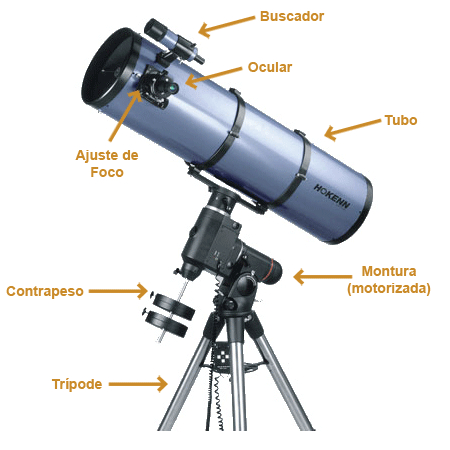
\includegraphics[width=0.5\textwidth]{./imagenes/telescopio}
\caption{Telescopio Astronómico (http://blog.astroaficion.com/)} \label{fig:telescopio}
\end{figure}

El telescopio es un instrumento cuya función principal es recoger la luz de un objeto lejano y ampliarlo. Está considerado como el artífice de la astronomía moderna.

Históricamente se le atribuye el descubrimiento a Hans Lippershey que era un fabricante de lentes, alemán, que también era científico, astrónomo e inventor.
Cuando Galileo Galilei escuchó la noticia de la creación del telescopio, decidió diseñar y construir uno, y en 1609 lo registró como el primer telescopio astronómico. Gracias a él, se pudo llevar a a cabo la destacada observación del día 7 de enero de 1610 donde se pudieron observar la existencia de cuatro de las lunas de Júpiter girando entorno al planeta.
En un principio el nombre que se le puso al instrumento fue de “lente espía”, y el 14 de abril de 1611 Giavanni Demisiani propuso el nombre de telescopio durante una cena que se brindó en honor a Galileo. Galileo decidió llevar a esa cena el telescopio y los comensales pudieron observar las lunas de Júpiter. El nombre por el que se conoce este instrumento, Telescopio, proviene del griego con el prefijo tele que significa “lejos” y se le añade la raíz griega skop que significa “ver”.

Además de poder ampliar los objetos lejanos para verlos con mayor detalle, gracias al telescopio se pueden observar cuerpos celestes de débil luminosidad y que son invisibles a simple vista, ya que el objetivo del telescopio es capaz de percibir más luz que el ojo humano. Cuanto mayor es el diámetro del objetivo, más luz capta. Dicho diámetro suele referenciarse como la “apertura del telescopio” y de ello depende el poder que tenga de resolución el objetivo y por tanto el telescopio.

Los primeros telescopios que se consolidaron fueron los de tipo kepleriano que disponían de unas longitudes focales de hasta 30 o 40 centímetros, con el objetivo de conseguir grandes aumentos.
A principios del siglo XVIII comenzaron a fabricarse los telescopios con lente y un espejo cóncavo a su vez. A partir de ese momento comenzó un debate sobre los telescopios, su utilidad y cual de ellos ofrecía mayor precisión, ya que existían dos tipos, los telescopios reflectores, en los que la luz es reflejada y dirigida hacia el foco, y los telescopios refractores, en donde  la luz es refractada pasando por el objetivo.
A mediados del siglo XX se terminó la disputa cuando triunfaron de manera definitiva los telescopios reflectores.

\subsection{Cámara CCD}
\begin{figure}[htb]
\centering
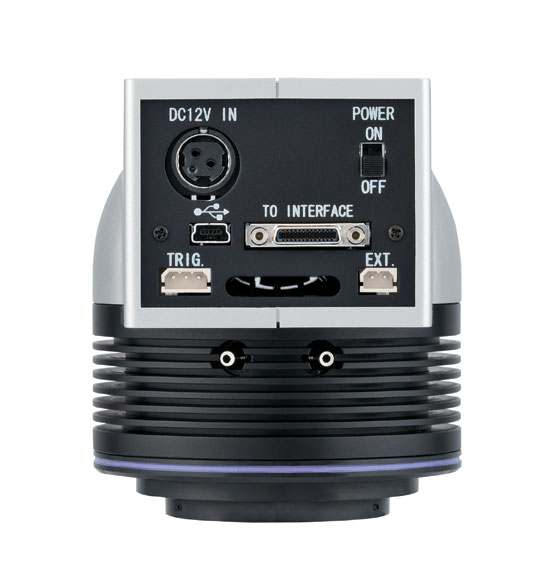
\includegraphics[width=0.4\textwidth]{./imagenes/ccd}
\caption{Cámara CCD (http://bitran.co.jp/)} \label{fig:ccd}
\end{figure}
Las siglas de cámara CCD (\textit{Charge-Coupled Device}) proceden del inglés y significan dispositivo de carga acoplada. Los primeros dispositivos que se crearon fueron inventados por Willard Boyle y George E. Smith, el 17 de octubre de 1969 dentro de los laboratorios Bell y ambos fueron distinguidos recientemente con el Premio Nobel de Física, en el año 2009, gracias a los dispositivos CCD.

Dicha cámara funciona como un detector de estado sólido. Este funcionamiento hace que la cámara sea muy eficiente ya que hace mucho más fácil la obtención y el procesamiento de las imágenes astronómicas.
La cámara CCD funciona como un conjunto de circuitos eléctricos  de condensadores enlazados y acoplados que son sensibles a la radiación electromagnética. Estos condensadores pueden transferir su carga eléctrica a uno o varios condensadores que se encuentren a su lado en el circuito impreso. El CCD registra la ubicación de cada fotodiodo sobre el que incide un fotón de rayos X. Un fotón es un paquete que contiene radiación electromagnética. A su vez, el CCD es capaz de registrar la energía que depende de su frecuencia, y por tanto, de su longitud de onda.

Los sensores CCD tienen una estructura de células que son sensibles a la luz en forma de mosaico y a cada una de esas células se le llama \textit{píxel}. Cada \textit{píxel} es una estructura detectora en la cual se pueden almacenar fotones. Desde el CCD la imagen es procesada por la cámara y a su vez registrada en la tarjeta de memoria.


\subsection{Montura}
\begin{figure}[htb]
\centering
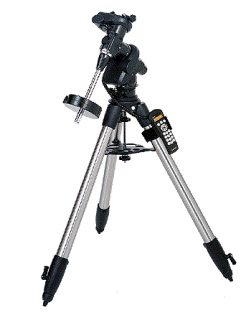
\includegraphics[width=0.5\textwidth]{./imagenes/montura}
\caption{Montura (http://astrofacil.com/)} \label{fig:montura}
\end{figure}
La montura es la parte mecánica. Sirve como estructura para montar y sujetar el tubo del telescopio y así poder realizar la operación de enfoque para poder detectar y seguir a un cuerpo celeste. Se requiere que la montura sea de mucha firmeza y a su vez tenga mucha suavidad en los movimientos para poder conseguir que las observaciones sean perfectas.

Existen varios tipos de monturas entre las que destacan: Altacimutales y Ecuatoriales.

La montura altacimutal es aquella que hace referencia al sistema de coordenadas celestes altacimutales. Requiere un continuo ajuste ya que tienen absoluta libertad para moverse en altura (de arriba hacia abajo) y en acimut (de derecha a izquierda).

La montura ecuatorial es aquella que hace referencia al sistema de coordenadas celestes ecuatoriales. Tiene un eje ecuatorial que está alineado con el eje terráqueo y algunas de estas monturas pueden disponer de un pequeño motor capaz de realizar un giro completo en 24 horas. Dispone además de otro eje, llamado declinación y es regular al primero.
Cuando se encuentra enfocado un astro y el motor se ha accionado, el tubo del telescopio sigue automáticamente el movimiento de la bóveda celeste y el objeto enfocado permanecerá fijo en el interior del campo visual del telescopio. Por este motivo tan importante, la montura ecuatorial es muy eficaz en la astronomía ya que permite exposiciones muy prolongadas.


\subsection{Enfocador}
\begin{figure}[htb]
\centering
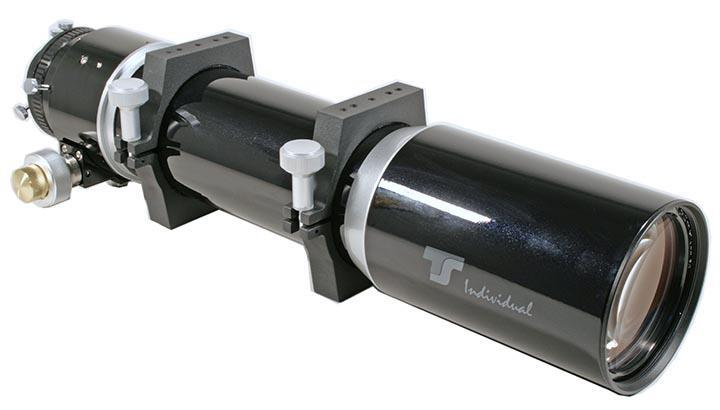
\includegraphics[width=0.5\textwidth]{./imagenes/enfocador}
\caption{Enfocador (http://tienda.lunatico.es/)} \label{fig:enfocador}
\end{figure}
El enfocador es una de las piezas fundamentales del telescopio ya que gracias a él, nos permitirá ver las imágenes formadas tras la reflexión de la luz en el espejo primario y su desviación por el espejo secundario.

Para ver las imágenes se necesitará un juego de oculares. La combinación de la longitud focal de los oculares y la longitud focal del telescopio, nos dará como resultado el número de aumentos total que tenemos en nuestro sistema.

Uno de los enfocadores más populares que existe actualmente en el mercado es el de tipo \textit{Crayford}. Estos enfocadores son bastante caros ya que tienen una relación de velocidad alta que mejora el ajuste de enfoque.


\subsection{Rueda Portafiltros}
\begin{figure}[htb]
\centering
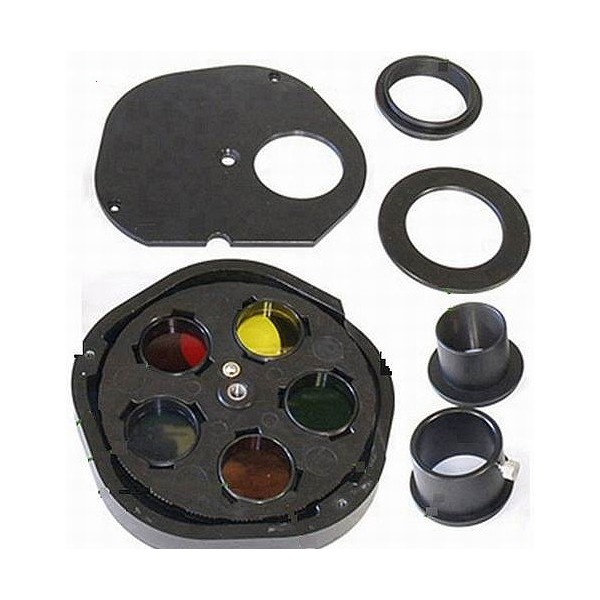
\includegraphics[width=0.5\textwidth]{./imagenes/ruedaPortafiltros}
\caption{Rueda Portafiltros (http://astrocity.es/)} \label{fig:ruedaPortafiltros}
\end{figure}
La rueda portafiltros es un objeto, generalmente de aluminio, que contiene en su interior filtros diferentes para poder cambiar de forma eficaz la visual o la astrofotografía. No hace falta quitar la cámara para cambiar el filtro ya que tan solo con un pequeño giro en la rueda se selecciona el filtro poniéndose en el lugar correcto y se puede seguir observando.
Como mínimo, se requiere que tenga cuatro filtros si se quiere realizar astrofotografía con cámaras CCD blanco y negro. Para ello, se necesitarán el filtro azul, el filtro rojo y el filtro verde (RGB), y posiblemente un filtro para los infrarrojos.


\subsection{Cúpula}
\begin{figure}[htb]
\centering
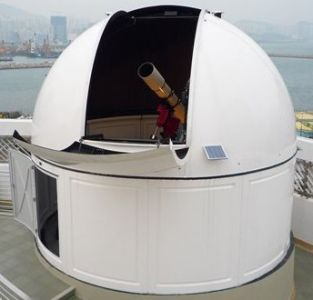
\includegraphics[width=0.4\textwidth]{./imagenes/cupula}
\caption{Cúpula Astronómica (http://apt.com.es/)} \label{fig:cupula}
\end{figure}
Una cúpula es una estructura principalmente semiesférica o de techo deslizante. La cúpula permite alojar en su interior el instrumental astronómico y protegerlo. Ya sea de un tipo o de otro, está formada por una o más escotillas que permiten su abertura y, de esta forma, poder realizar una observación.


\subsection{Óptica Adaptativa}
\begin{figure}[htb]
\centering
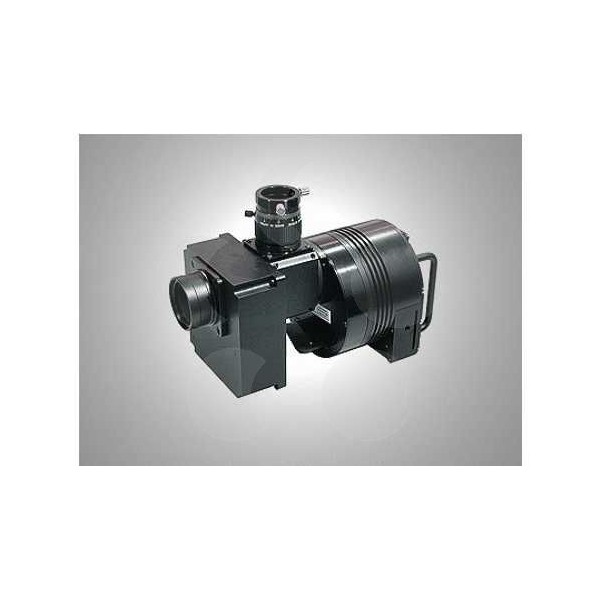
\includegraphics[width=0.3\textwidth]{./imagenes/opticaAdaptativa}
\caption{Óptica Adaptativa (http://www.valkanik.com/)} \label{fig:opticaAdaptativa}
\end{figure}
La óptica adaptativa es una técnica que permite, mediante el uso de óptica deformable, corregir en tiempo real los defectos que vienen de la atmósfera terrestre en la imagen observada con el telescopio. Es una técnica muy importante para todos los astrónomos ya que se pueden obtener imágenes mucho más nítidas. Un símil que hacen muchos astrónomos para entender esto es que la técnica es comparable con mirar un objeto situado en el fondo de una piscina con agua y sin agua.
La óptica adaptativa es capaz de eliminar las perturbaciones y por tanto equivaldría a observar desde el espacio. Ganar nitidez con la óptica en las imágenes significa concentrar en un menor número de puntos sensibles del detector los pocos fotones que llegan de los objetos débiles o lejanos y eso es, dicho con otras palabras, que la posibilidad de verlos es mayor.


\subsection{Estación Meteorológica}
\begin{figure}[htb]
\centering
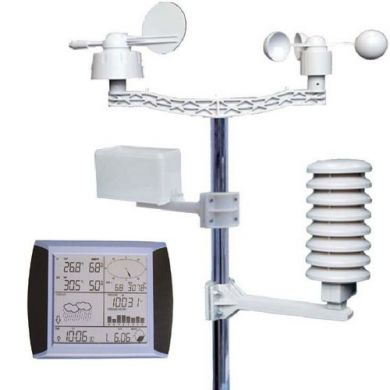
\includegraphics[width=0.4\textwidth]{./imagenes/estacionMeteorologica}
\caption{Estación Meteorológica (http://comprawifi.com/)} \label{fig:estacionMeteorologica}
\end{figure}
Una estación meteorológica es una instalación cuya función principal es medir y registrar diversos datos meteorológicos. Dichos datos se utilizan para elaborar predicciones meteorológicas a partir de modelos numéricos.
A su vez, la estación está formada por sensores e instrumentos que sirven para la obtención de todos los datos entre los que destacan el termómetro, el barómetro, el pluviómetro, el psicómetro o la veleta.


\subsection{Controlador de Dispositivos}
Hoy en día, en los observatorios, se pueden controlar los diversos instrumentos de un observatorio de diferentes formas como pueden ser:

  \begin{itemize}
    \item Controlados directamente desde el propio dispositivos.
    \item Mediante el uso de un PC y desde ahí se controlarían todos los aspectos.
    \item Mediante el uso de herramientas de control remoto. En este caso situarían al astrónomo en un lugar fuera del observatorio y desde ese lugar se podrían controlar los diferentes dispositivos que permitan realizar el trabajo del astrónomo.
  \end{itemize}


\section{Plataformas para la creación de \textit{software} astronómico}
Actualmente existen dos grandes protocolos para la creación de \textit{software} astronómico. Estos dos claros protocolos son ASCOM e INDI.  La función de ambos protocolos es llegar a poder controlar  todo el instrumental astronómico desde una misma máquina.

\section{ASCOM}
El protocolo ASCOM está formado por un conjunto de desarrolladores y fabricantes de instrumentales astronómicos. Lo que buscan lograr es la compatibilidad plug-and-play, independientemente del lenguaje que se utilice entre el \textit{software} y los instrumentos astronómicos. Para ello, crean una capa para separar los dispositivos del \textit{software} que utilizan los dispositivos. Otro objetivo es conseguir hacer que cualquier driver pueda ser utilizado en cualquier lenguaje de programación.

Tiene un gran inconveniente y es que actualmente solo funciona en sistemas operativos de \textit{Microsoft Windows} y dificulta su desarrollo ya que solamente está abierto a un único sistema operativo.

Por otra parte, hay que detallar que ASCOM no está pensado para funcionar remotamente pues su función está pensada para hacer escritorio remoto desde un sistema operativo de \textit{Microsoft Windows}.\cite{ASCOM}


!!!!!!!!!!!!!!!!!!!!IMPORTANTE!!!!!!!!!!!!!!!!!!!!
(PONER REFERENCIA A LA WEB DE ASCOM PARA ENGANCHAR CON LA BIBLIOGRAFIA)  (http://www.ascom-standards.org/)

\section{INDI}
INDI es un protocolo de \textit{software} libre diseñado para apoyar el control, la automatización, la adquisición de datos y el intercambio entre los dispositivos \textit{hardware} y las interfaces \textit{software}. Se puede usar tanto en dispositivos reales como en dispositivos virtuales.

Su biblioteca permite controlar cualquier dispositivo con un driver INDI mediante el paso de archivos del tipo XML.

INDI significa “\textit{Instrument-Neutral-Distributed-Interface}”. INDI fue creado por \textit{Elwood C. Downey} del \textit{ClearSky Institute}.

\subsection{Cómo funciona INDI}
Hoy en día, los sistemas de control que se desarrollan se hacen para una gama de dispositivos concretos o incluso para un dispositivo específico. Si se modifica algún parámetro del dispositivo o de la gama de dispositivos, el \textit{software} debe modificarse para asentar dicho cambio. En otras palabras, hay una fuerte conexión entre el \textit{software} y el \textit{backend} del \textit{hardware}.

Para que no exista esa fuerte conexión entre el \textit{software} y el \textit{backend} del \textit{hardware} se desarrolla INDI,  ya que los clientes son totalmente conscientes de las capacidades de los diferentes dispositivos que tienen conectados a través del protocolo INDI. Esto hace que en tiempo de ejecución, se construya una interfaz gráfica en función a las características que envíe el dispositivo. Dicha interfaz por tanto, se construye de forma dinámica.

\begin{figure}[htb]
\centering
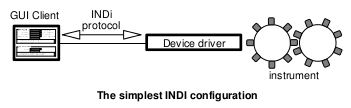
\includegraphics[width=0.6\textwidth]{./imagenes/funcionINDI}
\caption{Configuración de INDI (http://indilib.org/)} \label{fig:funcionINDI}
\end{figure}

Para que INDI funcione con total perfección se definen tres sustantivos muy importantes que hacen que encajen todas las piezas correctamente. Estos sustantivos son: \textit{drivers}, servidor y cliente.

\subsection{\textit{Drivers}, Servidores y Clientes de INDI}
\begin{itemize}
  \item El \textit{driver} de INDI es un controlador que se comunica directamente con el dispositivo. Permite conectarse a uno o más dispositivos físicos y es el responsable de definir todos los clientes. Los \textit{drivers} envían una lista de propiedades a los clientes para que éstos puedan así definir dinámicamente sus interfaces gráficas.
  \item El servidor es un programa que ejecuta los diferentes \textit{drivers} de los distintos dispositivos. Hace de conexión entre los dispositivos y los clientes. Por regla general está alojado en un ordenador en el cual están todos los dispositivos conectados. También el servidor permite que estén los dispositivos conectados en otras máquinas y éstas envíen los datos al servidor.
 Todo el intercambio de datos que se realiza entre el servidor y los \textit{drivers} se consigue mediante el uso del protocolo INDI.
  \item El cliente es un programa que hace dinámicamente la interfaz gráfica. Puede estar conectado con uno o más servidores. Una vez que conecta con uno o más servidores el cliente solicita toda la información y el servidor se la da. Seguidamente, el cliente procesa los datos y los muestra creando la interfaz que se menciona anteriormente.
\end{itemize}

\subsection{Descripción del protocolo}
El protocolo INDI define un conjunto de 5 propiedades que son las que envían los diferentes \textit{drivers} para formar la interfaz del cliente. Estas propiedades están muy relacionadas ya que una o todas las propiedades pueden estar presentes en un dispositivo. A continuación se pasa a detallar cada una de las propiedades:
\begin{itemize}
  \item \textbf{Textos:} Son cadenas de caracteres ordenados arbitrariamente.
  \item \textbf{Números:} Son cantidades numéricas. Además de la cantidad numérica se envían otros parámetros que sirven para el formato de su visualización y configuración.
  \item \textbf{Switchs:} Son propiedades que están encendidas o apagadas. Estas propiedades pueden ser de tres tipos diferentes:
    \begin{itemize}
      \item \textbf{Una de muchas:} de todas las opciones se tiene que seleccionar obligatoriamente una.
	    \item \textbf{Como máximo una:} de todas las opciones se puede seleccionar como máximo una.
	    \item \textbf{Cualquiera de muchas:} se podrán seleccionar todas las que se deseen.
    \end{itemize}
  \item \textbf{Lights:} Son propiedades que pueden estar en cada uno de los cuatro estados que se definen:
    \begin{itemize}
      \item \textbf{Inactivo:} Luz de color gris.
      \item \textbf{Alerta:} Luz de color rojo.
      \item\textbf{Ocupado:} Luz de color amarillo.
      \item \textbf{Ok:} Luz de color verde.
    \end{itemize}
  \item \textbf{Blob:} Son propiedades que tienen objetos binarios arbitrariamente, como imágenes.
\end{itemize}

\subsection{Simuladores}
INDI dispone de un conjunto de simuladores que sirven para testear todo lo que se va haciendo sin necesidad de tener un dispositivo físico. Con él se pueden realizar todo tipo de operaciones sin variar nada con respecto al dispositivo real. Entre ellos destacan:
\begin{itemize}
  \item Simulador de telescopio.
  \item Simulador de CCD.
  \item Simulador de rueda portafiltros.
  \item Simulador de enfocador.
  \item Simulador de GPS.
\end{itemize}

\section{Estado del arte. \textit{Software} con INDI y sin él}
Actualmente existen diferentes \textit{softwares} para realizar la función control de un observatorio. Hay que destacar que podemos diferenciarlos en dos grandes grupos: Los \textit{softwares} que no hacen uso de la biblioteca INDI y los que si hacen uso de dicha biblioteca.

\subsection{Clientes que no hacen uso de INDI}
\begin{itemize}
  \item \textbf{Maxim DL:} Dispone de una completa integración del observatorio y controla todo el equipo astronómico. Es compatible con ASCOM y el astrónomo puede crear sus propios preajustes. A su vez, se puede supervisar y controlar el observatorio mediante una webcam en la cúpula, interruptores remotos y vigilancia del clima. Es uno de los software sin INDI más completo que existe.
  \item \textbf{Images Plus:} Es un \textit{software} que en un principio sirve para realizar el tratamiento de astrofotografía pero que después se ha ido mejorando y hoy en día permite hacer uso y control de dispositivos. Su uso es muy limitado ya que solamente permite hacer uso de algunos dispositivos concretos. También funciona con ASCOM.
  \item \textbf{Astroplanner:} Permite planificar y ejecutar una sesión de observación al astrónomo. Se pueden introducir los sitios que se desean observar, importarlos desde archivos o buscar en el catálogo del que dispone el programa. Se puede usar tanto en MAC OS X (10.4 o superior) y en \textit{Windows} (XP o superior). Funciona también con ASCOM en la versión para \textit{Windows} pero solamente para el control de telescopios.
\end{itemize}
Referencias de los tres puntos anteriores(respectivamente):
(http://www.cyanogen.com/maximmain.php)
(http://www.mlunsold.com/ILControl.html)
(http://www.astroplanner.net/requirements.html)

\subsection{Clientes que hacen uso de INDI}
\begin{itemize}
  \item \textbf{KStars:} Es una herramienta de \textit{Software Libre} de astrofotografía incluida en multiplataforma. Proporciona una simulación gráfica precisa del cielo nocturno desde cualquier punto de la tierra. Además, proporciona herramientas de cálculo astronómico y mucha información que ayudará y facilitará el trabajo  al astrónomo.
  \item \textbf{Ekos:} Software que lleva a cabo tareas de astrofotografía bajo la plataforma Linux. Ekos es también una herramienta de \textit{Software Libre} y forma parte del \textit{software} de Kstars mencionado anteriormente.
  \item \textbf{\textit{Remote Observatory}:} Es un cliente INDI multilenguaje de \textit{Software Libre} para la plataforma Android. Se encuentra en un continuo desarrollo y permite controlar cualquier número de servidores así como múltiples interfaces.
\end{itemize}
Referencias de los tres puntos anteriores(son la misma):
http://www.indilib.org/about/clients.html

Como conclusión final diremos, que vistos algunos de los clientes que se pueden usar para llevar a cabo el control de un observatorio hay que resaltar que ninguno de ellos es capaz de llevar dicho control desde el navegador, y por tanto, necesitaríamos de un pc con unos requerimientos mínimos puesto que todos los pcs que existen en la actualidad los superarían, y una instalación del \textit{software} que, en nuestro caso, seleccionásemos.
Pruebas

%
\chapter{Objetivos}
\title{Objetivos}
\label{cap:Objetivos}

El objetivo fundamental de este proyecto es desarrollar un prototipo de cliente web basado en INDI que sea capaz de realizar la función control sobre un observatorio astronómico. Dicho prototipo será multiplataforma y utilizará tecnologías de carácter \textit{Software Libre}. Se pretende además, que en la medida de lo posible se añadan nuevas funcionalidades en un futuro y que se convierta en un cliente web y no en un prototipo.


\section{Objetivos Principales y Secundarios}
A continuación se detallan los objetivos principales del prototipo del cliente web:

\begin{itemize}
  \item \textbf{OBJ-1:} Crear un prototipo de cliente que sea capaz de realizar el control de cualquier dispositivo INDI sin apreciar su naturaleza.
  \item \textbf{OBJ-2:} Permitir la conexión con un servidor concreto mediante su IP y su puerto.
  \item \textbf{OBJ-3:} Efectuar la gestión de múltiples dispositivos que estén conectados a un servidor.
  \item \textbf{OBJ-4:} Desarrollar un prototipo de cliente multiplataforma, que permita hacer uso del prototipo del cliente en los principales navegadores que existen en el mercado.
  \item \textbf{OBJ-5:} Utilizar \textit{Software Libre} en la aplicación como herramienta de trabajo.
  \item \textbf{OBJ-6:} Ofrecer la posibilidad de que cualquier desarrollador pueda aportar su capacidad y conocimiento al prototipo.
  \item \textbf{OBJ-7:} Aportar una nueva forma de acceder a los datos de un observatorio astronómico.
  \item \textbf{OBJ-8:} Optimizar el uso de instrumentos de astronomía facilitando una nueva herramienta de obtención de datos.
\end{itemize}

Por otra parte, se busca conseguir los siguientes objetivos secundarios:

\begin{itemize}
  \item \textbf{OBJ-S-1:} Adaptar el prototipo de cliente web a las propiedades estándares de INDI.
  \item \textbf{OBJ-S-2:} Adecuar el prototipo a los estándares de HTML, CSS, Jquery y JavaScript.
  \item \textbf{OBJ-S-3:} Desarrollar el prototipo de modo que funcione correctamente con el mayor número posible de dispositivos conectados al servidor.
  \item \textbf{OBJ-S-4:} Conseguir que la interfaz sea maximizable y minimizable independientemente del número de dispositivos conectados al servidor.
  \item \textbf{OBJ-S-5:} Difundir el prototipo de cliente web en la página web de INDI.
  \item \textbf{OBJ-S-6:} Divulgar el prototipo de cliente web en el foro de INDI
\end{itemize}


\section{Materias y Herramientas para el Desarrollo}
Este trabajo no se hubiera podido desarrollar sin haber obtenido unos conocimientos básicos y en profundidad en las siguiente materias:
\begin{itemize}
  \item Fundamentos de la Ingeniería del Software para realizar el análisis y la ingeniería de requisitos.
  \item Infraestructuras Virtuales para realizar el conjunto de pruebas y simulaciones.
  \item Transmisión de Datos y Redes de Computadores para configurar las conexiones y la red a la hora de hacer uso del prototipo.
  \item Tecnologías Web para poder realizar una web en HTML y darle un estilo propio con CSS.
  \item Programación Web para poder complementar aún más la materia de Tecnologías Web.
  \item Diseño de Aplicaciones para Internet para desarrollar una aplicación multiplataforma y que funcione en cualquier ordenador con conexión a internet.
\end{itemize}

Por último, hay que hacer mención a los importantes e imprescindibles conocimientos obtenidos en otros campos como:
\begin{itemize}
  \item Astronomía, para entender todo lo que se va buscando en ella.
  \item Equipos astronómicos, para entender cómo funcionan y los resultados que se esperan de ellos.
  \item Websocket, para establecer un canal bidireccional entre el cliente y el servidor.
  \item SublimeText, para poder desarrollar el código fuente del trabajo.
  \item LaTeX, para poder realizar la documentación del proyecto.
  \item GitHub, para realizar un control de versiones del proyecto tanto en la parte de desarrollo del código fuente como en la parte de desarrollo de la documentación.
  \item GanttProject, para realizar los diferentes diagramas de Gantt \cite{DiagramaGantt} usados en la planificación.
\end{itemize}


\section{Alcance de los Objetivos}
El prototipo de cliente web debe cumplir con todos los objetivos específicos que más arriba exponemos y que nos hemos planteado ante el reto que supone este trabajo. El que así sea es de relevante importancia dado que actualmente no existe ningún cliente web basado en INDI para controlar un observatorio astronómico.

Así mismo, una vez que se finalice el proyecto, se desea concluir con el prototipo y que pase a ser un cliente web estable y que los profesionales y estudiosos en la materia que nos ocupa puedan hacer uso y disfrute del mismo.

Esta es una de las razones principales por las que se ha desarrollado este prototipo. Se ha desarrollado bajo \textit{Software Libre} con la intención de que cualquier desarrollador pueda continuar con el proyecto bajo los estándares de \textit{Software Libre}.

Por otra parte, se intentará que dicho prototipo sea publicado en la página web oficial de INDI para que los diferentes usuarios puedan verlo, interesarse y contribuir a su desarrollo final.


\section{Interdependencia de los Objetivos}
El objetivo fundamental y que se debe conseguir con este proyecto es el \textbf{OBJ-1} ya que es el desarrollo del prototipo de cliente web basado en INDI.

Todos los objetivos planteados tienen entidad propia e independencia en sí mismo, exceptuando los objetivos secundarios \textbf{OBJ-S-1} y \textbf{OBJ-S-2}, de relevante importancia, puesto que seguir los estándares hará que se optimice notablemente el funcionamiento del prototipo.

%
\chapter{Planificación}
\title{Planificación}
\label{cap:Planificacion}

Este proyecto se ha planificado siguiendo los puntos que a continuación se detallan y que permiten trabajarlo de una manera ordenada a la vez que dan información al lector facilitándole una visión amplia y exhaustiva, así como la comprensión de la posterior exposición del mismo. A continuación se detallan los diferentes puntos de la planificación que han sido estudiados para este proyecto

\section{Metodología de Desarrollo}
La metodología utilizada ha sido el modelo iterativo que es el que más y mejor se ajusta a las características del proyecto. La elección de este tipo de metodología se justifica por los siguientes aspectos de la misma:

\begin{itemize}
  \item Permite un entendimiento incremental del proyecto.
  \item Habilita una fácil retroalimentación al usuario.
  \item Dispone de objetivos parciales y metas concretas.
  \item El proceso es medido conforme avanzan todas las implementaciones.
\end{itemize}

\begin{figure}[htb]
\centering
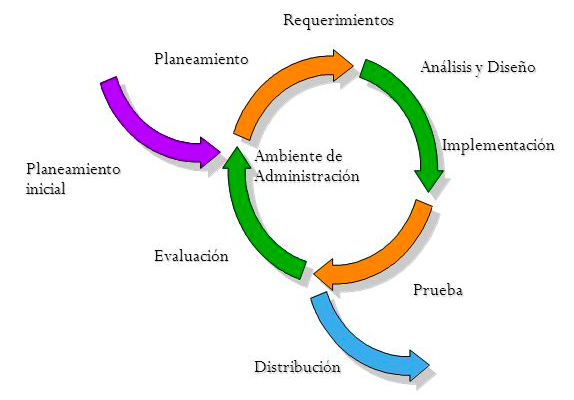
\includegraphics[width=1\textwidth]{./imagenes/modeloIterativo}
\caption{Modelo Iterativo (http://adsi.foroactivo.com//)} \label{fig:modeloIterativo}
\end{figure}

Además de la utilización del modelo iterativo que por sus características específicas es el más idóneo para este trabajo, hay que mencionar que para el control de versiones del proyecto se ha estado utilizando el software Git y para guardar los datos se ha recurrido al servicio GitHub.

\section{Fases}
En este punto se van a exponer de manera más exhaustiva y se va a entrar en detalle, cada una de las fases que se desarrollan para completar el proyecto viéndose, de esta forma, el progreso del mismo.

\subsection{Planteamiento del Problema}
\begin{itemize}
  \item Descripción: Exposición del problema que se desea resolver, pautas a seguir y familiarización con las tecnologías.
  \item Apartado: Capítulo \ref{cap:Introduccion}.\\
\end{itemize}

\subsection{Especificaciones del Proyecto}
\begin{itemize}
  \item Descripción: Obtención de los requisitos funcionales y requisitos no funcionales del proyecto.
  \item Apartado: Capítulo \ref{cap:Analisis}.\\
\end{itemize}

\subsection{Planificación}
\begin{itemize}
  \item Descripción: Estimación temporal, estimación de costes económicos y estimación de recursos humanos.
  \item Apartado: Capítulo \ref{cap:Planificacion}.\\
\end{itemize}

\subsection{Ingeniería}
\begin{itemize}
  \item Descripción: Análisis de los requisitos y diseño del sistema a desarrollar.
  \item Apartado: Capítulos \ref{cap:Analisis} y \ref{cap:DisenoEImplementacion}.\\
\end{itemize}

\subsection{Construcción}
\begin{itemize}
  \item Descripción: Implementación del proyecto.
  \item Apartado: Capítulo \ref{cap:DisenoEImplementacion}.\\
\end{itemize}

\subsection{Pruebas}
\begin{itemize}
  \item Descripción: Pruebas internas del proyecto
  \item Apartado: Capítulo \ref{cap:Pruebas}.\\
\end{itemize}


\section{Estimación Temporal}
Seguidamente se hace una estimación temporal del proyecto detallando cada una de las fases de la sección anterior.

\begin{itemize}
  \item \textbf{Planteamiento del Problema:}
  \begin{itemize}
    \item Descripción de los objetivos a grandes rasgos.
    \item Comprender el protocolo INDI.
    \item Entender los diferentes instrumentos que intervendrán en el protocolo.
    \item Planteamiento de las posibles tecnologías que se usarán en el proyecto.
  \end{itemize}
\end{itemize}
\textit{\textbf{Estimación: 20 horas.}}\\ \\

\begin{itemize}
  \item \textbf{Especificaciones del Proyecto:}
  \begin{itemize}
    \item Conocer perfectamente las necesidades del usuario.
    \item Establecer los objetivos que deben plantearse ante este proyecto.
    \item Extracción de los requisitos funcionales.
    \item Extracción de los requisitos no funcionales.
  \end{itemize}
\end{itemize}
\textit{\textbf{Estimación: 30 horas.}}\\ \\

\begin{itemize}
  \item \textbf{Análisis y Diseño:}
  \begin{itemize}
    \item Análisis de los requisitos que debe reunir este proyecto.
    \item Diagramas del proyecto.
    \item Metodología empleada en el desarrollo del proyecto
  \end{itemize}
\end{itemize}
\textit{\textbf{Estimación: 40 horas.}}\\ \\

\begin{itemize}
  \item \textbf{Construcción:}
  \begin{itemize}
    \item Establecimiento de las herramientas, las plataformas, los diferentes tipos de lenguajes y el \textit{software} que se va a utilizar
    \item Creación de la interfaz para conectarse a un servidor INDI concreto mediante su IP y su puerto.
    \item Creación de la interfaz para mostrar en una ventana el dispositivo con sus grupos y sus diferentes propiedades.
    \item Creación de la interfaz para mostrar, en la pantalla, varias ventanas con diferentes dispositivos conectados al servidor simultáneamente.
    \item Posibilidad de cambiar cualquier parámetro de un dispositivo conectado.
    \item Posibilidad de enviar información al servidor con los parámetros que hayan sido modificados.
  \end{itemize}
\end{itemize}
\textit{\textbf{Estimación: 110 horas.}}\\ \\

\begin{itemize}
  \item \textbf{Pruebas:}
  \begin{itemize}
    \item Pruebas de integración.
    \item Pruebas de sistema.
    \item Pruebas de aceptación.
  \end{itemize}
\end{itemize}
\textit{\textbf{Estimación: 10 horas.}}\\ \\


\begin{itemize}
  \item \textbf{Documentación:}
  \begin{itemize}
    \item Documentación del código del prototipo del cliente.
    \item Documentación del proyecto.
    \item Manual de usuario del prototipo.
  \end{itemize}
\end{itemize}
\textit{\textbf{Estimación: 40 horas.}}\\


\begin{table}[h]
\centering
\label{table:tiempoEstimado}
\begin{tabular}{ll}
\hline
{\bf Tarea a realizar}                   & {\bf Tiempo estimado (horas)} \\ \hline
Planteamiento del problema    & 20 horas                            \\
Especificaciones del proyecto & 30 horas                            \\
Análisis y diseño             & 40 horas                            \\
Construcción                  & 110 horas                           \\
Pruebas                       & 10 horas                            \\
Documentación                 & 40 horas                            \\
{\bf Total}                   & {\bf 240 horas}                           \\ \hline
\end{tabular}
\caption{Estimación temporal}
\end{table}


\section{Recursos Humanos}
Gracias a que se ha elegido en la realización y posterior utilización de este proyecto un \textit{Software Libre}, toda persona que tenga unos conocimientos mínimos en programación, astronomía e INDI, que desee realizar una aportación puede hacerlo en el \href{https://github.com/PabloTorrecillas/IndiWebClient}{repositorio del proyecto}.

El desarrollo del proyecto ha sido realizado por una única persona y, que en este caso, coincide con el autor del presente documento.

Como para la realización del proyecto, desde su inicio hasta la finalización del mismo, se han utilizado unos 4 meses aproximadamente, se podría decir que el proyecto realizado por una única persona supondría un trabajo desarrollado a lo largo de un periodo de cuatro meses. Por el contrario, si se dispusiera de un equipo formado por cuatro personas, se obtendría el mismo resultado con una duración de un mes.

\section{Recursos \textit{Software} Reutilizables}
Los siguientes recursos hacen mención a diferentes desarrollos software creados por otras empresas o por otros desarrolladores.

Como el objetivo fundamental del proyecto es la creación de un prototipo de cliente web capaz de controlar un observatorio astronómico desde cualquier lugar del planeta donde exista conexión a internet, se tendrán que tener en cuenta durante el desarrollo, todas aquellas herramientas que permitan realizar el prototipo HTML y aquellas bibliotecas de software libre que se encuentran en internet. Dichas bibliotecas se podrán consultar y utilizar, tanto para añadir funcionalidad al prototipo de cliente, como para realizar los diferentes elementos gráficos del proyecto.

\section{Estimación de Costes Económicos}
En esta sección se va a proceder a la estimación de todos los costes económicos para poder llevar a cabo el proyecto:

\subsection{Licencias \textit{Software}}
Dado que el proyecto se realiza mediante herramientas de desarrollo de \textit{Software libre} no es necesario realizar el pago de ninguna licencia \textit{software}.

\subsection{Recursos Humanos}
Representan la totalidad de personas que forman el equipo y que han contribuido al desarrollo y finalización de este proyecto. El tiempo que se ha empleado para este trabajo arroja un total de 240 horas.

Dado que la ley prohíbe de forma expresa a los Colegios de Profesionales para disponer e informar sobre los honorarios, se tomarán como honorarios a percibir el sueldo medio que recibiría un Graduado en Ingeniería Informática. Partiendo de esta premisa, se hará una estimación de que el precio por hora será de unos 18\euro. El resultado final que se obtiene analizando el coste económico del equipo de trabajo, en este proyecto, sería la cantidad de 4320\euro.

\subsection{Material}
Dado que INDI dispone de diferentes simuladores con los que poder realizar todas las pruebas necesarias para comprobar que el prototipo de cliente funciona, el coste total del material ha sido de 0\euro.

Por otra parte, se puede utilizar una cámara \textit{reflex nikon D3200} con un objetivo 18-55mm valorada en 339,99\euro según Amazon.\cite{NikonAmazon}

Por último, no se le puede restar al material un elemento imprescindible y de vital importancia para este proyecto como es un ordenador. Gracias al ordenador se podrá llevar a cabo la función de programación, documentación del código, buscar información, etcétera. El precio aproximado es de 450\euro.

Como conclusión, en cuanto a la estimación de costes económicos referidos a la realización de este proyecto, obtenemos los siguientes resultados:
\\ \\
\begin{table}[h]
\centering
\label{table:costeEstimado}
\begin{tabular}{ll}
\hline
{\bf Gastos}                   & {\bf Coste Estimado en euros} \\ \hline
Licencias \textit{software}   & 0\euro                             \\
Recursos humanos              & 4320\euro                          \\
Material                      & 790\euro                           \\
{\bf Total}                   & {\bf 5110\euro}                          \\ \hline
\end{tabular}
\caption{Estimación de coste económico}
\end{table}


\section{Temporización}
Se ha elaborado una estimación temporal acorde a las tareas realizadas en la sección de estimación temporal y atendiendo también al número de días. Para mostrarlo de una forma más sencilla, se ha creado un diagrama de Gantt.

\begin{figure}[htb]
\centering
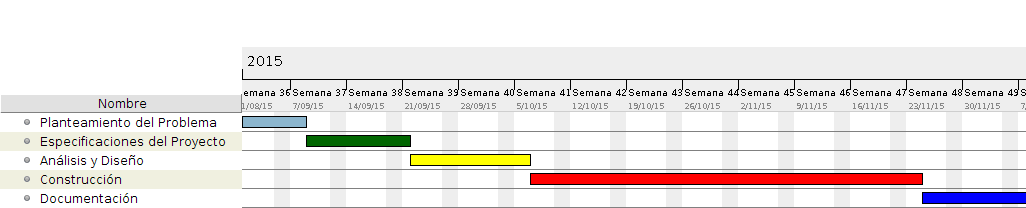
\includegraphics[width=1\textwidth]{./imagenes/proyectoGantt}
\caption{Diagrama de Gantt} \label{fig:proyectoGantt}
\end{figure}

%
\chapter{Analisis}
\title{Analisis}
\label{cap:Analisis}

En este capitulo se realizará un análisis del proyecto para poder hacer así el futuro diseño del mismo.
Se describirán las diferentes partes que se han desarrollado.

\section{Análisis de Requisitos}
El análisis de los requisitos es el conjunto de todas las tareas que formarán las distintas necesidades de un software. Todos estos requisitos se tomarán por parte tanto del cliente como del desarrollador del proyecto ya que tiene que existir una viabilidad en el proyecto.

Se realiza un análisis de requisitos para que al llegar a la fase de diseño se tenga un software óptimo, sin contradicciones o sin ambigüedades, por ejemplo.

Los requisitos se van generando a partir de las diferentes entrevista que se tienen con el cliente.

\subsection{Requisitos Funcionales}
\begin{itemize}
  \item \textbf{RF-1:} Conectarse a un servidor INDI.
  \item \textbf{RF-2:} Mostrar todos los dispositivos conectados en el servidor INDI.
  \item \textbf{RF-3:} Obtener las propiedades de los dispositivos conectados.
  \item \textbf{RF-4:} Agrupar las propiedades de los dispositivos por diferentes grupos.
  \item \textbf{RF-5:} Editar las diferentes propiedades de INDI:
  \begin{itemize}
    \item \textbf{RF-5.1:} Propiedad Text.
    \item \textbf{RF-5.2:} Propiedad Number.
    \item \textbf{RF-5.3:} Propiedad Switch.
    \item \textbf{RF-5.4:} Propiedad Blob.
    \item \textbf{RF-5.5:} Propiedad Light.
  \end{itemize}
  \item \textbf{RF-6:} Activar la recepción de Blob en cada dispositivo conectado.
  \item \textbf{RF-7:} Desactivar la recepción de Blob en cada dispositivo conectado.
\end{itemize}

%
\chapter{Diseño e Implementación}
\title{Diseño e Implementación}
\label{cap:DisenoEImplementacion}
Este proyecto se realiza atendiendo a dos partes, ambas muy importantes y claramente diferenciadas. Por una parte, se ha creado el diseño del prototipo de cliente y por otra parte se ha elaborado el boceto de la interfaz con su posterior diseño de interfaz de usuario.

\section{Diagrama del Modelo Conceptual}
El diagrama del modelo conceptual nos ofrece una idea de cómo se encuentra interrelacionadas las diferentes entidades del sistema.
\begin{figure}[htb]
\centering
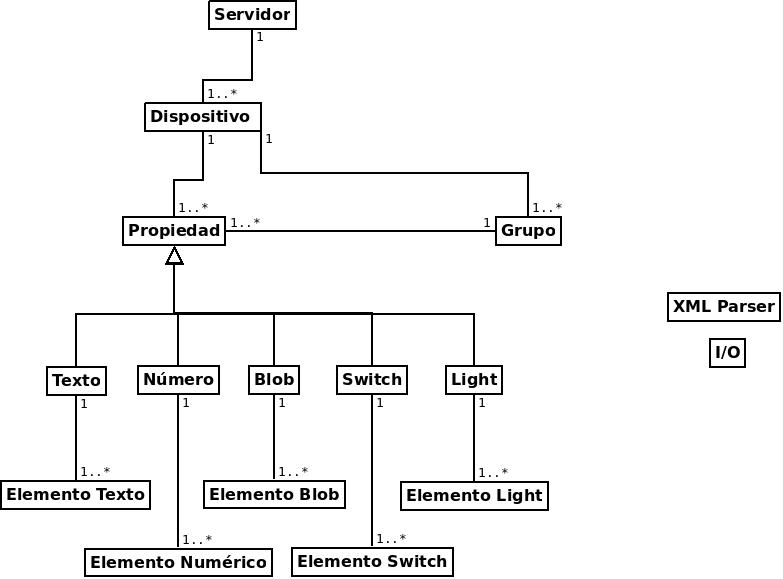
\includegraphics[width=0.8\textwidth]{./imagenes/diagramaConceptual}
\caption{Modelo Conceptual} \label{fig:diagramaConceptual}
\end{figure}

Como se puede observar en el diagrama, en un servidor se pueden encontrar uno o muchos dispositivos conectados en él.
A su vez, un dispositivo puede tener un conjunto de propiedades y un conjunto de grupos. Las propiedades solamente pueden pertenecer a un grupo concreto.\\
Cada propiedad es solamente de un tipo, que puede ser \textit{text}, \textit{number}, \textit{switch}, \textit{blob} y \textit{light}. A su vez, la propiedad puede tener uno o muchos elementos de dicha propiedad.\\

Por último, hay que destacar que se han creado las entidades \textit{XML Parser} y \textit{I/O}, para el parseo de los mensajes enviados por el servidor en \textit{XML} y para la entrada y salida, respectivamente.


\section{Diseño del Prototipo del Cliente}
El diseño del prototipo del cliente es la pieza fundamental del proyecto ya que sobre dicho prototipo giran todas las cosas.\\

La función principal del prototipo es permitir conectarnos con cualquier servidor INDI y una vez que establecemos la conexión, mediante el WebSocket, es fundamental que la comunicación se establezca de forma continua con el fin de recibir los diferentes dispositivos que se encuentran conectados con el servidor en concreto y así poder intercambiar mensajes con los parámetros que se van modificando en ambas partes.

\subsection{Métodos en el Fichero \textit{connection.js}}
El cometido de estos métodos es establecer la conexión con el servidor.
También, en ese archivo, se pueden encontrar los métodos para poder realizar el envío de valor de los parámetros modificados, ya sea de tipo \textit{text}, \textit{number}, \textit{switch} o \textit{blob}, al servidor mediante el \textit{WebSocket}, que se crea en el momento de la conexión.

\subsection{Métodos en el Fichero \textit{parserDefVector.js}}
Este fichero se establece en dos grandes bloques. En primer lugar, se encuentran los métodos mediante los cuales se va creando la interfaz con los datos que se reciben del fichero XML, como pueden ser, entre otros, los nombres de los dispositivos, los nombres de las propiedades, los apelativos de los grupos de las propiedades, los valores que tienen dichas propiedades, etc. En segundo lugar, se hallan las funciones auxiliares para crear dicha interfaz y que sirven de apoyo a los métodos de análisis y parseo de las propiedades.\\

Una vez que llegan esos datos se crean las diferentes ventanas que corresponden a cada dispositivo siempre y cuando estos dispositivos no estén ya creados.
Tanto para las propiedades de \textbf{texto} como para las de \textbf{número} se realiza el mismo proceso.\\

A continuación, se pone una bombilla del color correspondiente según el estado que envíe el fichero XML que proviene del servidor, y el nombre de la propiedad. Este conjunto se ha denominado \textit{propertyBox}.
Seguidamente, mediante el parseo del fichero XML, se va recorriendo cada uno de los nodos que lo van formando y para cada uno de ellos se muestra el nombre que viene descrito mediante el campo \textit{label} y su correspondiente valor del nodo. Al conjunto formado por el nombre y el valor se le ha denominado \textit{elementBoxContainer}.\\

Posteriormente, y según el tipo de permiso que tenga esa propiedad, se pone o no el botón de actualizar para que en el futuro se puedan modificar los campos y poder así enviarle el mensaje al servidor.\\

Por último, se añade a las diferentes pestañas la propiedad, según el grupo al que pertenece la propiedad que se está analizando.\\

Para el análisis y posterior parseo de la propiedad \textbf{\textit{switch}} se sigue el mismo itinerario con el que se ha procedido en los \textit{text} y en los \textit{number}, con la diferencia de que en la parte del \textit{elementBoxContainer}, se hacen diferentes tipos de llamadas para cada una de las diferentes reglas  que pueden contener las propiedades \textit{switch}:
\begin{itemize}
  \item \textbf{\textit{One Of Many:}} se crea un desplegable que siempre obliga al usuario a tener una opción seleccionada en ella.
  \item \textbf{\textit{At Most One:}} se crea un desplegable que permite al usuario si así lo desea o le es factible, solo seleccionar una de todas las opciones que se muestran en él.
  \item \textbf{\textit{Any Of Many:}} se crea un conjunto de opciones que le permitirán al usuario seleccionar todas las que se deseen.
\end{itemize}
Según el tipo de permiso que tenga esa propiedad, se dispone o no, el botón de actualizar para que en el futuro se puedan modificar los campos y poder enviarle el mensaje al servidor.\\

Para el análisis y parseo de la propiedad \textbf{\textit{blob}}, se ha seguido también el mismo procedimiento que en las diferentes propiedades pero en este caso, se ha hecho una pequeña variante en la parte del \textit{elementBoxContainer}. Dentro de ella se muestra, igualmente, el nombre y el valor de la propiedad y además, se añaden dos campos nuevos que son el tamaño del \textit{blob} y su correspondiente formato.
De igual forma, en su parte derecha, y siempre dependiendo  del tipo de permiso que corresponda, se añade o no el botón de actualizar para enviar los datos al servidor.\\

En último lugar, hay que decir que en la parte del análisis y su correspondiente parseo sobre la propiedad \textbf{\textit{light}}, se realiza lo mismo que en las diferentes propiedades salvo en el \textit{elementBoxContainer} que se añade el nombre de la propiedad y el color de la bombilla correspondiente al valor que se envía en ese nodo.\\

Hay que destacar que esta propiedad es siempre del tipo solo lectura y por tanto, no se agregará nunca un botón ya que no se pueden cambiar los valores que tiene.\\

Por otra parte, hay que destacar los métodos auxiliares para la creación del interfaz. Estos métodos son de igual o más importancia que los anteriores ya que sin ellos no se podrían crear las ventanas, poner los diferentes tipos de interruptores o incorporar las diferentes pestañas a las ventanas de los dispositivos.\\

\subsection{Métodos en el Fichero \textit{parserSetVector.js}}
Están constituidos por un total de cinco métodos, uno para cada una de las diferentes propiedades que dispone INDI.
La función principal de estos cinco métodos es común a todos y es la de almacenar los diferentes valores que se cambian en el prototipo de cliente para poder enviárselos al servidor.
Actualmente, en el prototipo, la función de envío se está realizando sobre los propios botones, sobre los desplegables o sobre los \textit{checkbox} que se han ido creando dinámicamente en el fichero anterior. En esos botones se realiza la llamada que corresponda al envío según la propiedad y se hace todo el envío desde el fichero connection.js como se ha mencionado anteriormente.

\subsection{Métodos en el Fichero \textit{parser.html}}
Es el punto de partida de todo el proceso. Desde ahí se establece la conexión con el servidor y se crea un bucle mediante el cual se va enviando la información a las diferentes funciones según el tipo de propiedad que se esté recibiendo o enviando.
También dispone de un conjunto de funciones auxiliares que son comunes tanto a \textit{parserDefVector.js} como a \textit{parserSetVector.js}. Estas pueden ser, por ejemplo, el obtener el nombre de las funciones o conseguir lograr el tipo de bombilla a poner, entre otras.

\section{Bocetos de la Interfaz}
La interfaz de usuario es el medio con que el usuario puede comunicarse, en este caso, con la computadora mediante su navegador y comprende todos los puntos de contacto entre el usuario y el equipo. Por regla general, suelen ser fáciles de entender y fáciles de interactuar con ellas, aunque en el ámbito de la informática es preferible referirse a ellas como que suelen ser “amigables e intuitivas” porque es complejo a la vez que  subjetivo, nombrarlas con el adjetivo “fácil”.\cite{IU}\\

A lo largo de cada una de las diferentes iteraciones del proceso se han ido mejorando las interfaces ya que se ha ido incrementando el número de elementos y por tanto, cada vez había que hacer la interfaz con un grado de dificultad añadido.\\

En la primera iteración se elaboró todo el diseño en papel para ir constituyendo un esquema de lo que sería la futura la interfaz de usuario.\\
\begin{figure}[htb]
\centering
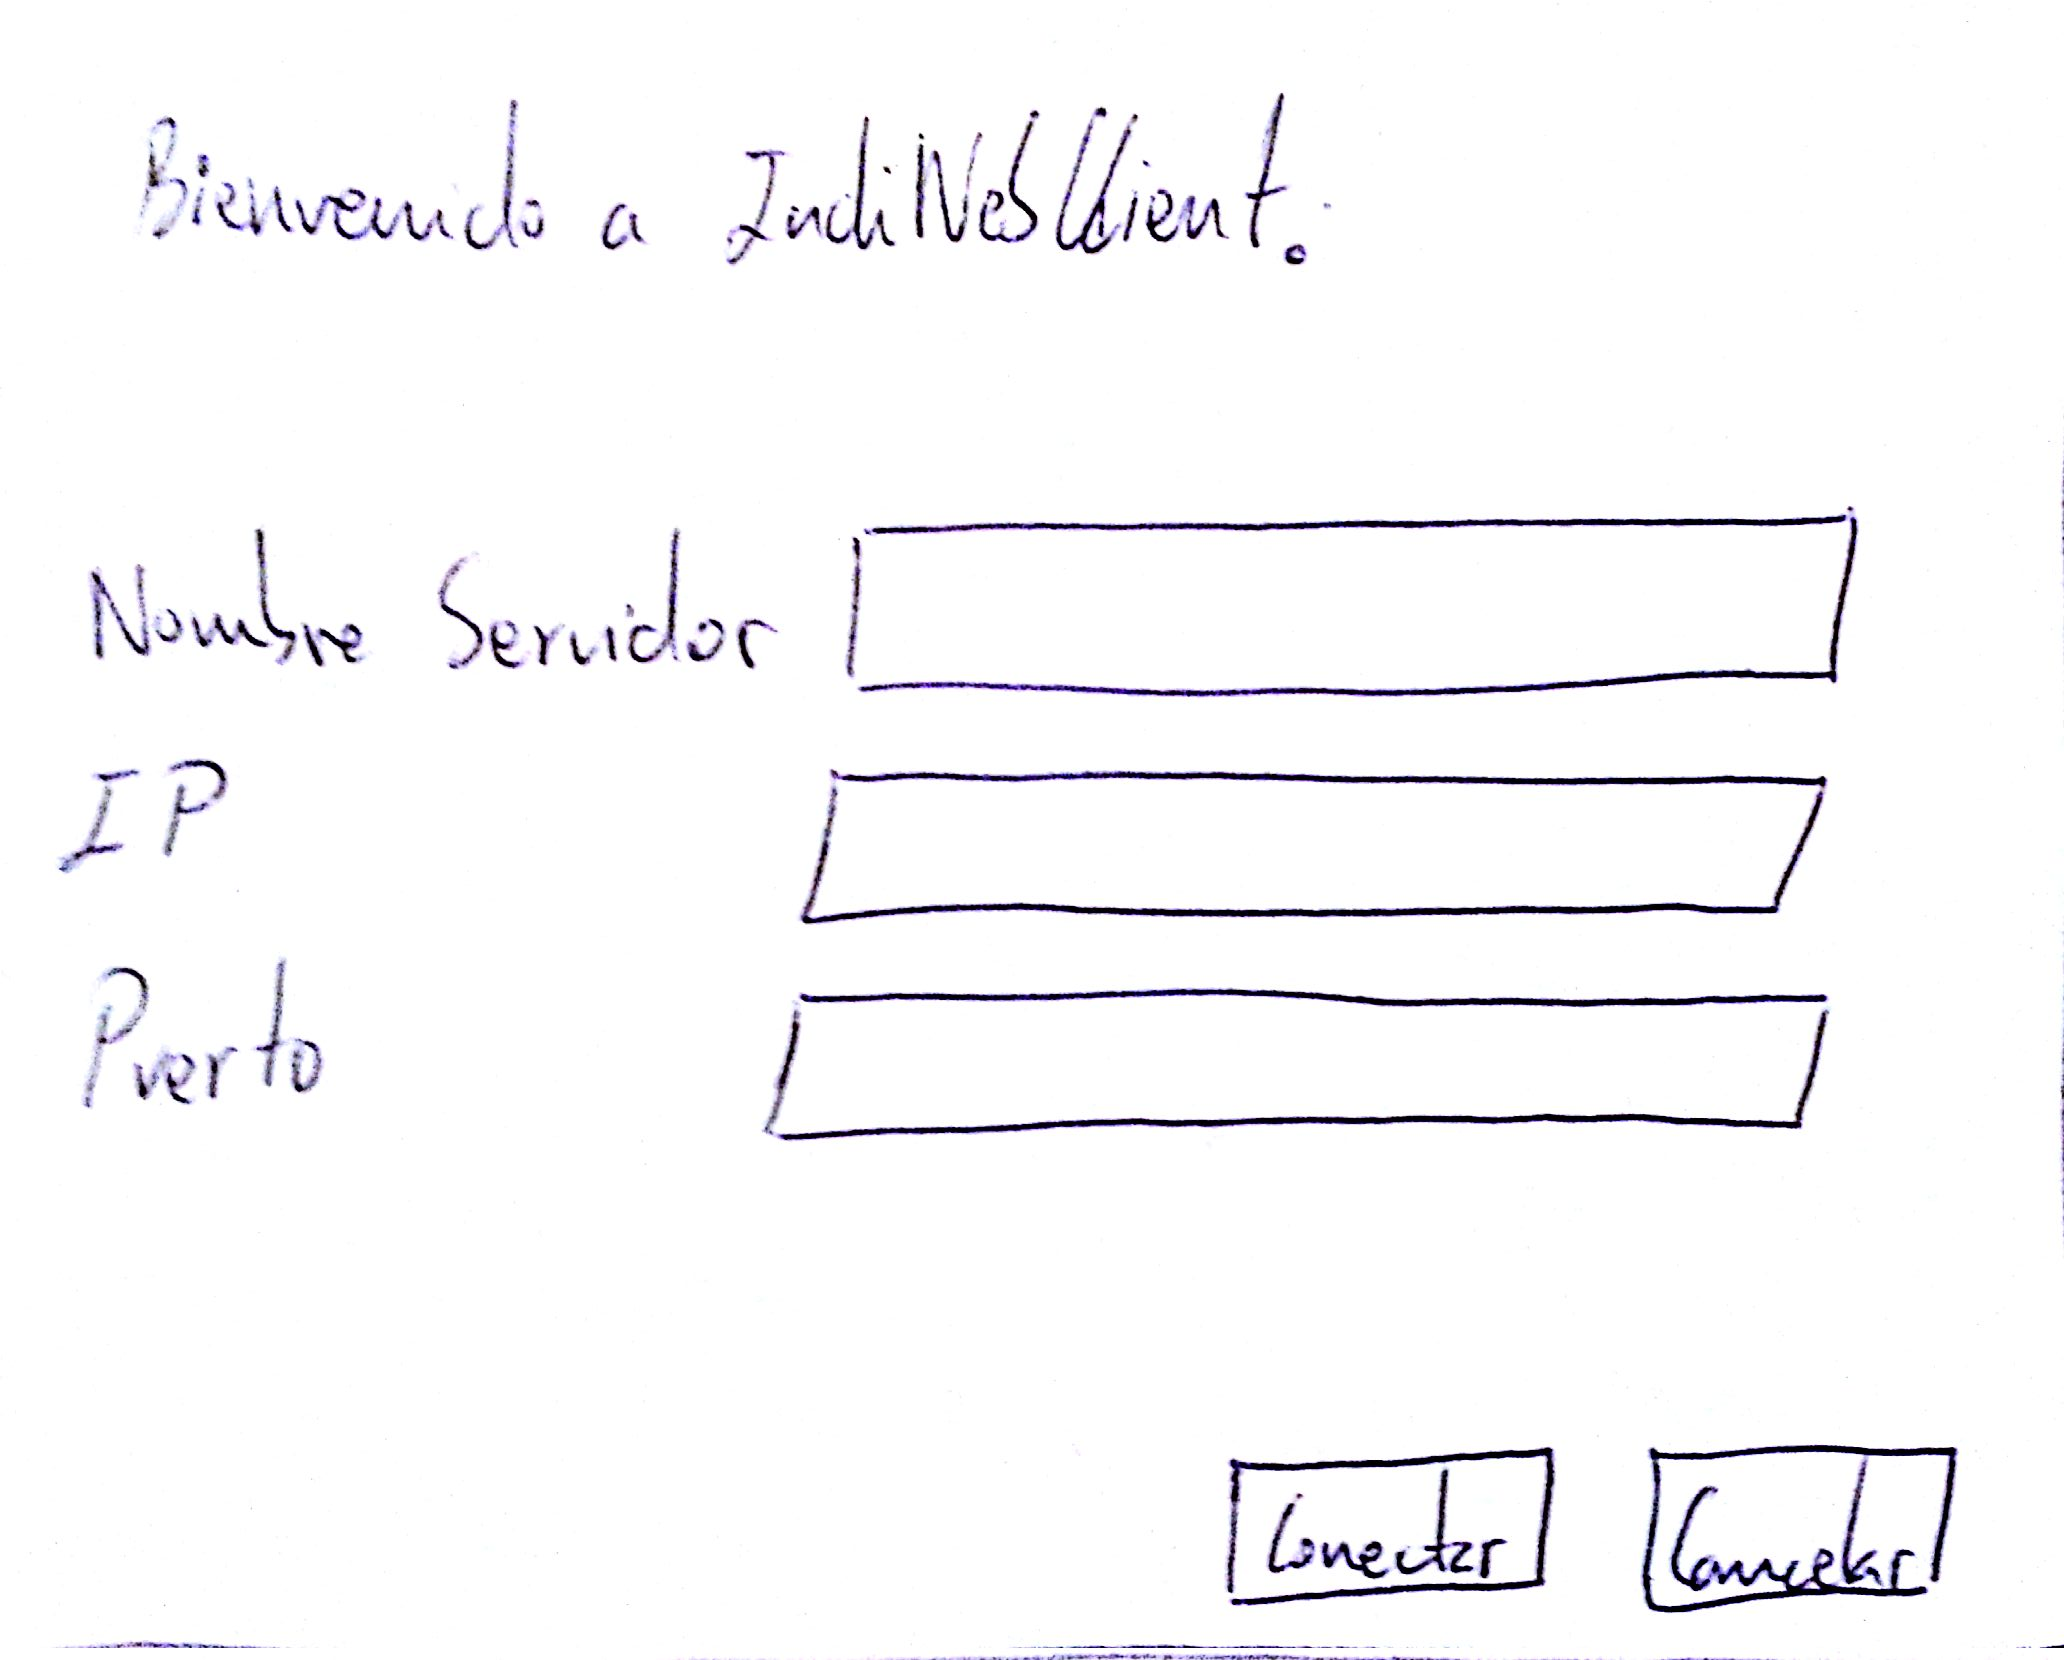
\includegraphics[width=0.7\textwidth]{./imagenes/boceto1}
\caption{Boceto de la Interfaz (I)} \label{fig:boceto1}
\end{figure}

\begin{figure}[htb]
\centering
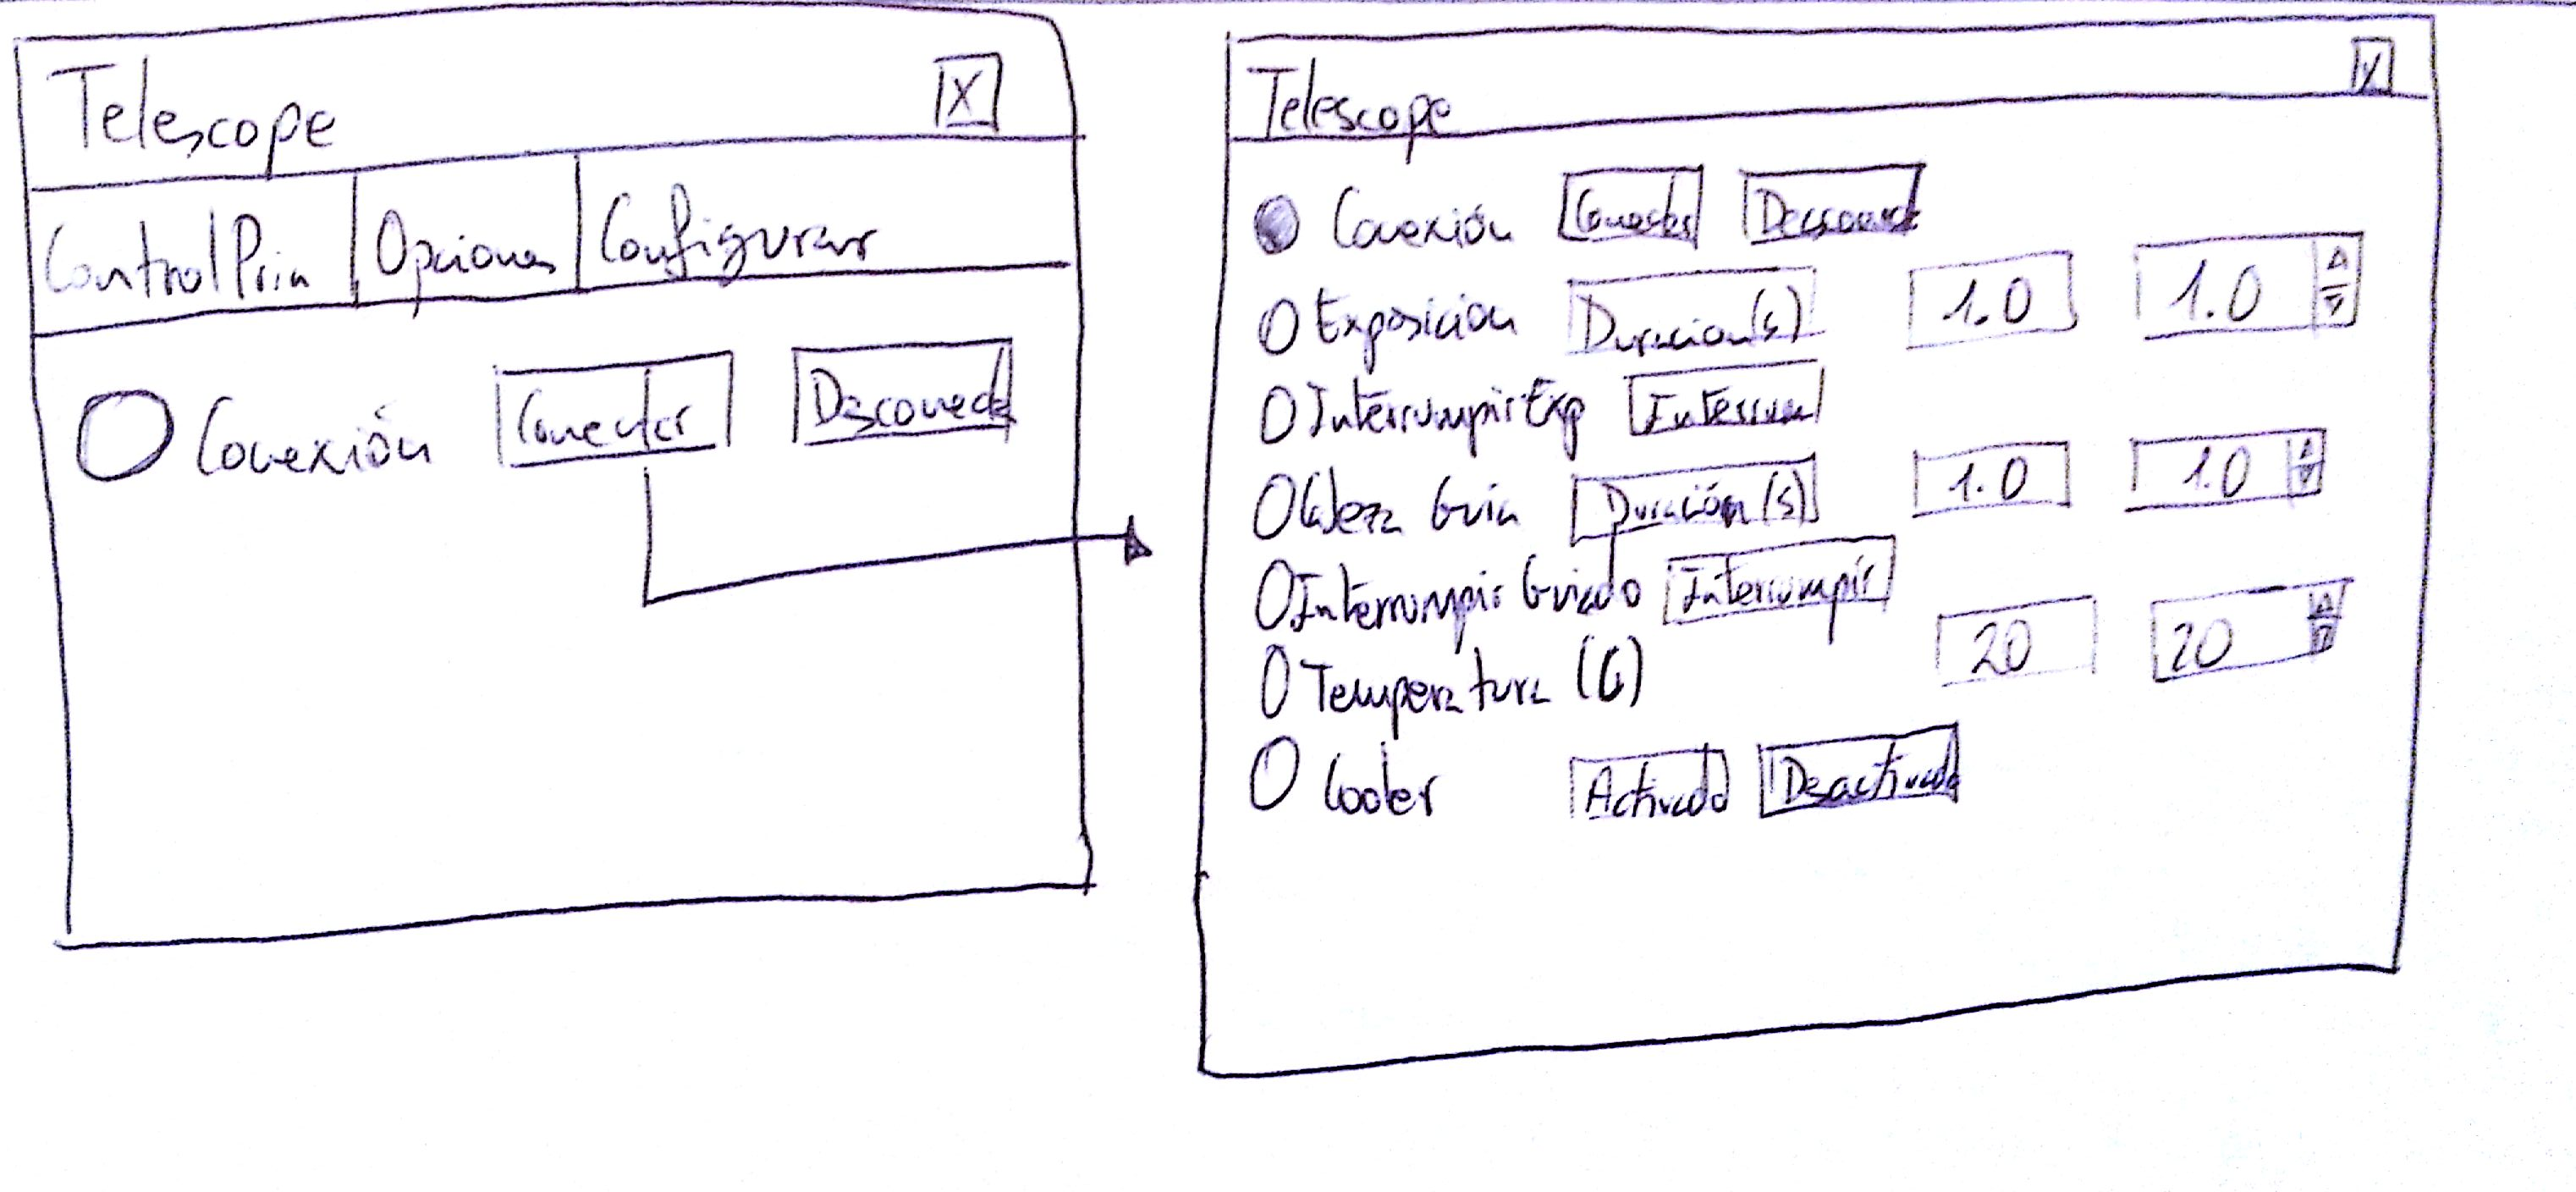
\includegraphics[width=1\textwidth]{./imagenes/boceto2}
\caption{Boceto de la Interfaz (II)} \label{fig:boceto2}
\end{figure}

Seguidamente, y en las iteraciones posteriores, se comenzó a plasmar el trabajo del papel en el navegador comenzando a crear las primeras ventanas para ir proyectando como colocar los diferentes elementos que las iban a integrar.

\begin{figure}[htb]
\centering
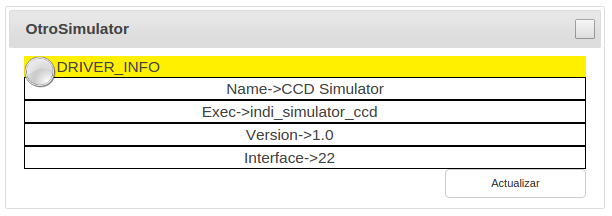
\includegraphics[width=1\textwidth]{./imagenes/primerasVentanas1}
\caption{Primeras Ventanas de la IU (I)} \label{fig:primerasVentanas1}
\end{figure}

\begin{figure}[htb]
\centering
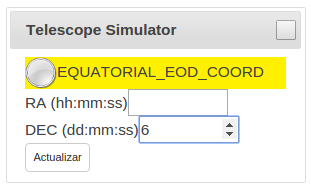
\includegraphics[width=0.7\textwidth]{./imagenes/primerasVentanas2}
\caption{Primeras Ventanas de la IU (II)} \label{fig:primerasVentanas2}
\end{figure}

Posteriormente, se consiguió el diseño final de la interfaz del prototipo del cliente web.\\ \\

\begin{figure}[htb]
\centering
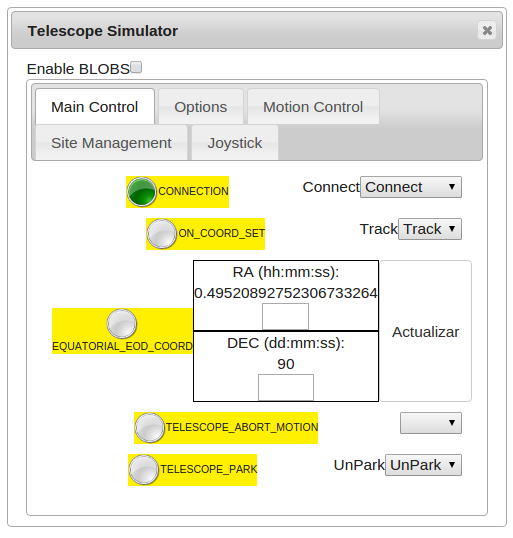
\includegraphics[width=0.8\textwidth]{./imagenes/interfazActual}
\caption{Interfaz de Usuario Actual de Dispositivo} \label{fig:interfazActual}
\end{figure}

\section{Diseño de la Interfaz}
Para obtener unos mejores resultados, se han ido desarrollando las interfaces por separado:
\begin{itemize}
  \item Interfaz de conexión.
  \item Interfaz de propiedad.
  \item Interfaz de grupo de elementos.
  \item Interfaz de dispositivo.
\end{itemize}

\subsection{Interfaz de Conexión}
Se define como la pantalla principal del prototipo de cliente. En ella se muestran dos cuadros de texto para introducir la IP y el puerto del servidor con el que se desea conectar.

\subsection{Interfaz de Propiedad}
Es una interfaz que tendrá, aproximadamente para cada propiedad, la misma estructura.
En la parte izquierda se observa como aparece la bombilla del estado de la propiedad y seguidamente su nombre. A continuación, se encuentra el nombre y el valor de la propiedad o nombres y valores, dependiendo de si tiene más de uno. Por último se encuentra el botón de actualizar, para el caso de que su permiso lo permita.\\

Para los \textit{switch} en la parte central, seguido de la bombilla y el nombre, se encontrará el desplegable con las diferentes opciones o casillas para marcar, según el caso de  su regla de \textit{switch}, ya  sea una u otra.\\

Para los \textit{blob}, su parte central, estará formada por el nombre y el valor, y además existirán dos campos extra que serán el tamaño y el formato del propio \textit{blob}.\\

Para los \textit{light}, en su parte central, se encontrará una o más bombillas con su correspondiente nombre cada una.

\subsection{Interfaz de Grupos de Propiedades}
La interfaz del grupo de propiedades comprende las diferentes pestañas según se agrupan las propiedades. Cuando llega un mensaje en \textit{XML} del servidor se analiza y se comprueba si para el dispositivo que ha enviado el mensaje hay ya creada una ventana, que en caso de no existir, se crea y a continuación el grupo se almacena como una pestaña en la cual irán todas las propiedades de ese grupo.
Se comprueba si la pestaña correspondiente a ese grupo existe y en caso de existir, se muestra la propiedad en esa pestaña. En caso contrario, si se da la circunstancia de que no existiera se crea una nueva pestaña y se muestra en ella la propiedad que envía en ese momento el servidor.\\

\subsection{Interfaz de Dispositivo}
Se entiende por interfaz de dispositivo la ventana encargada de mostrar toda la información del dispositivo conjuntamente con las diferentes interfaces precedentes descritas. En ella se pueden encontrar las diferentes propiedades de un dispositivo en cada una de las pestañas según correspondan a un grupo o a otro. Esta interfaz es la que se muestra cuando se realiza la conexión con el servidor INDI para cada uno de los dispositivos conectados. Es la interfaz que tiene mayor importancia puesto que en ella se muestra toda la información correspondiente al dispositivo.


\section{Implementación}
\subsection{Licencia}
Una de las principales características de este proyecto es que, desde un primer momento, se pensó en la elección de \textit{Software Libre} como herramienta y soporte para su desarrollo y posterior utilización. Se ha elegido  la licencia \textbf{GPL v3} por los siguientes motivos:

\begin{itemize}
  \item Es \textit{Software Libre}.
  \item Obliga a redistribuir con la misma licencia.
  \item Está aprobada por \textit{Open Source Initiative}.
  \item Se compromete y obliga a poder disponer del material de forma ilimitada y gratuita para toda aquella persona que lo solicite.
\end{itemize}

\subsection{Desarrollo de Código}
Para todo el desarrollo del código se ha utilizado el editor de textos y código Sublime Text\cite{Sublime}.
Las razones que hemos tenido para hacer esta elección han sido las siguientes: el tener un tamaño muy reducido, poseer un arranque casi inmediato y poder ampliar su funcionalidad a través de \textit{plugins}.

Este editor de textos y código no es gratuito. Eso es cierto, sin embargo, para el desarrollo de este proyecto que se presenta, he utilizado una versión de prueba que es de tiempo ilimitado.\cite{BeneficiosSublime}\\

Por otra parte, y para tener un control de versiones se ha utilizado \textit{Git}, así como para guardar los datos se ha recurrido al servicio \textit{GitHub}\cite{GitHub}.

Todo el código fuente se puede encontrar en el \href{https://github.com/PabloTorrecillas/IndiWebClient}{repositorio del proyecto}.

%
\chapter{Pruebas}
\title{Pruebas}
\label{cap:Pruebas}

En cada itereación de la planificación se han realizado una mínima parte de pruebas ya que al trabajar sobre un prototipo no se podía efectuar una batería de pruebas puesto que los resultados obtenidos podrían no ser los esperados. Es por ello, que las pruebas realizadas han sido pruebas internas y se ha procedido cuidando mucho los detalles en ellas para no entorpecer el funcionamiento del prototipo.\\

Las pruebas internas que se han materializado han sido las siguientes:
\begin{itemize}
  \item Pruebas de unitarias.
  \item Pruebas de integración.
  \item Pruebas de sistema.
  \item Pruebas de aceptación.
\end{itemize}

\section{Pruebas Unitarias}
Son aquellas pruebas que se han efectuado sobre módulos sencillos, sin estar conectados unos con otros y para verificar el resultado que se obtiene.

\subsection{Conexión con el servidor INDI}
\textbf{Objetivo de la prueba:} Comprobar que la conexión es correcta con el servidor INDI desde el prototipo de cliente que está usándose en el navegador del ordenador.\\

\textbf{Fases de la prueba:}
\begin{itemize}
  \item Conexión a un servidor INDI: Se conecta con el servidor INDI y se comprueba que el funcionamiento de la conexión es satisfactoria. El servidor recibe valores esperados y ejecuta correctamente.
  \item Conexión y finalización del servidor: Se comprueba cómo reacciona el prototipo de cliente cuando el servidor está caído. Se descubrió que el resultado que se obtenía al intentar cambiar algún tipo de parámetro en un dispositivo, era que no se almacenaban los valores ni respondía el servidor.
\end{itemize}

\subsection{Propiedades con el Servidor INDI}
\textbf{Objetivo de la prueba:} Comprobar que las propiedades funcionan correctamente dentro de los dispositivos con datos erróneos.\\

\textbf{Fases de la prueba:}
\begin{itemize}
  \item Datos fuera del rango establecido en la propiedad \textit{number}: Se prueba que el servidor no almacena un dato fuera del rango de una determinada propiedad.
  \item Datos en formato erróneo en la propiedad textit{number}: Se comprueba que el servidor no modifica datos en otro formato que no sea el que se le indica al poner el cursor sobre la casilla de modificación numérica y, por tanto, no los almacena.
\end{itemize}

\subsection{Grupos de Propiedades}
\textbf{Objetivo de la prueba:} Poder realizar diferentes pruebas con el conjunto de grupos de propiedades.

\textbf{Fases de la prueba:}
\begin{itemize}
  \item Mostrar diferentes grupos para un dispositivo: Se comprueba que se crean tantas pestañas como grupos de propiedades existen para un dispositivo.
  \item Añadir una propiedad nueva a un grupo de nueva creación: Se introduce una nueva pestaña y dentro de ella se almacena dicha propiedad.
  \item Añadir una propiedad nueva a un grupo previamente establecido: Se añade esa propiedad al grupo que ya está creado y al mismo tiempo se muestran los elementos que ya existen en él.
\end{itemize}

\section{Pruebas de Integración}
Las pruebas de integración realizadas han sido muy sencillas. En estas pruebas todos los módulos están interconectados unos con otros y se efectúan para comprobar que todas las conexiones están bien practicadas y, por consiguiente, se obtendrán unos resultados satisfactorios. Las diferentes pruebas de integración se han realizado con el servidor INDI sobre un simulador de telescopio. Para ello se han elaborado dos tipos de pruebas: Pruebas de conexión con el servidor y pruebas de manejo de las propiedades del dispositivo.

\subsection{Pruebas de conexión con el servidor}
\textbf{Objetivo de la prueba:} Conseguir que la función principal de esta prueba sea que el prototipo de cliente se conecte con el servidor sin ningún tipo de problema.

\textbf{Fases de la prueba:}
\begin{itemize}
  \item Se realiza la conexión con el servidor y a su vez con el simulador del telescopio. Como resultado se obtiene que se muestre el telescopio con todas sus propiedades y con sus grupos de propiedades. Al apagar el servidor, se comprueba cómo no se obtienen resultados por parte de éste y el envío de cambio de valores no se realiza puesto que no hay conexión. No se muestran mensajes si se aborta o falla la conexión.
\end{itemize}

\subsection{Pruebas de Manejo de las Propiedades del Dispositivo}
\textbf{Objetivo de la prueba:} Comprobar que todas las propiedades del dispositivo funcionan correctamente cuando se envían parámetros de las diferentes propiedades.

\textbf{Fases de la prueba:}
Para cada propiedad, se cambian algunos parámetros y se comprueba que el envío al servidor es satisfactorio y éste lo recepciona y modifica los parámetros enviados.

\begin{itemize}
  \item Propiedad \textit{Text}: Se cambia el texto de la propiedad y se comprueba que se realizó el cambio adecuadamente.
  \item Propiedad \textit{Number}: Se cambia el número por valores que sean correctos y se comprueba que el cambio ha sido positivo. Por otra parte, también se realizan dos comprobaciones más, una para el valor numérico fuera de rango y otra para el valor numérico con un formato incorrecto. Para ambas pruebas, se puede apreciar cómo no se envían los parámetros al servidor y cómo no se modifican dichos parámetros en el prototipo del cliente ya que no los trata como números correctos.
  \item Propiedad \textit{Switch}: Se sustituirán los parámetros de los diferentes \textit{switch} que de los que dispone el simulador del telescopio. Se puede apreciar, claramente, que no es posible introducirle valores erróneos ya que si la propiedad es, por ejemplo, de la regla de \textit{al menos uno}, siempre tendremos que seleccionar uno y no será posible dejarlo en blanco. Para las propiedades con la regla \textit{uno de muchos} o \textit{cualquiera de muchos}, tampoco es posible forzar a un error.\\
  Como resultado se comprueba que la propiedad \textit{switch} funciona correctamente en todos los aspectos.
  \item Propiedad \textit{Blob}: Se verifica que la recepción de \textit{blob} ha sido satisfactoria. No se muestra nada sobre ella, tan solo que se puede guardar.
\end{itemize}

Como \textbf{nota importante}, hay que destacar que para la \textbf{propiedad light} no se realizan pruebas de integración ya que es una propiedad del tipo solo lectura y no se puede interactuar con ella. Por supuesto, se ha realizado la prueba de comprobación de que si llega un mensaje XML del servidor INDI con una propiedad \textit{light}, dicha propiedad se muestra correctamente en la ventana del dispositivo del cual proviene.

%
%\input{capitulos/07_Pruebas}
%
%\chapter{Conclusiones}
\title{Conclusiones}
\label{cap:Conclusiones}

Una vez que se ha finalizado el desarrollo del proyecto, se evalúa el grado de consecución de los objetivos planteados  al inicio de este trabajo, y se observa que se han alcanzado en su totalidad, cada uno en su justa medida y atendiendo a su amplitud e importancia dentro del nivel que han ocupado en este trabajo. \\

Los objetivos más amplios y que se han conseguido trabajando en profundidad el tema han sido los objetivos principales del prototipo, y se han superado en su integridad, extensamente.
Los objetivos secundarios también se han conseguido en su totalidad. Debo hacer una salvedad respecto a dos de los objetivos secundarios planteados inicialmente, cuales son los objetivos secundarios para “la difusión del prototipo en la página web de INDI” y el objetivo secundario proyectado para “la divulgación del prototipo en el foro de la web de INDI”. Estas dos secciones del proyecto se han trabajado someramente porque se ha pensado que ambos apartados se alejaban o no eran imprescindibles en el tema central del proyecto, dejando la posibilidad a otros estudiosos del tema para su desarrollo. Por tanto, se puede decir que ambos objetivos se han conseguido en la medida en que se han trabajado esos apartados.\\

Puntualizado este extremo, determinamos que la evaluación final hay que calificarla como muy positiva, ya que se ha conseguido desarrollar un prototipo de cliente web haciendo combinación de varias tecnologías y ofreciendo al cliente un amplio abanico de posibilidades a realizar.\\

Por otra parte, cabe destacar en este cliente web, lo genuino, la originalidad y la innovación que representa su creación y desarrollo, puesto que actualmente no existe un cliente web capaz de alcanzar lo que si se consigue ejecutar en este prototipo de cliente, ser  capaz de realizar la función control de un observatorio, sea cual sea su localización, siempre que esté conectado a un servidor INDI y desde cualquier punto geográfico del planeta Tierra.\\

Como futuro cliente, debería:
\begin{itemize}
  \item Gestionar varias conexiones a diferentes servidores INDI.
  \item Posibilitar la desconexión de un servidor INDI.
  \item Desarrollar mecanismos de seguridad y privacidad en el cliente.
  \item Modificar la interfaz de usuario para hacerla más atractiva.
\end{itemize}

Por último hay que tener en cuenta un aspecto importante. Todas las pruebas que se han desarrollado en el prototipo de cliente han sido de carácter interno. Ninguna prueba ha sido documentada y todas las que se han realizado han sido para efectuar pequeñas comprobaciones y confirmar que no se habían recibido o enviado datos erróneos.\\

Como conclusión, hay que decir que el Prototipo de Cliente Web basado en INDI es susceptible de ser mejorado en más aspectos ya que está en sus inicios y se pretende conseguir que llegue a ser un cliente web fiable basado en INDI, a la vez de que sea capaz de realizar, en toda su extensión, la función control de observatorios que estén en cualquier parte del mundo y tengan un servidor INDI.\\

%
%%\chapter{Conclusiones y Trabajos Futuros}
%
%
%%\nocite{*}
\bibliography{bibliografia}\addcontentsline{toc}{chapter}{Bibliografía}
%\bibliographystyle{miunsrturl}
\bibliographystyle{plain}
%
%\appendix
%\input{apendices/manual_usuario/manual_usuario}
%%\input{apendices/paper/paper}
%\input{glosario/entradas_glosario}
% \addcontentsline{toc}{chapter}{Glosario}
% \printglossary
\chapter*{}
\thispagestyle{empty}

\end{document}
